\documentclass{wissdoc}
% Autor: Roland Bless 1996-2009, bless <at> kit.edu
% ----------------------------------------------------------------
% Diplomarbeit - Hauptdokument
% ----------------------------------------------------------------
%%
%% $Id: thesis.tex 65 2012-05-10 10:32:11Z bless $
%%
% wissdoc Optionen: draft, relaxed, pdf --> siehe wissdoc.cls
% ------------------------------------------------------------------
% Weitere packages: (Dokumentation dazu durch "latex <package>.dtx")
\usepackage[numbers,sort&compress]{natbib}
\usepackage{url}
\usepackage{amssymb}
%\usepackage{graphicx} 
% \usepackage{varioref}
% \usepackage{verbatim}
% \usepackage{float}    %z.B. \floatstyle{ruled}\restylefloat{figure}
% \usepackage{subfigure}
% \usepackage{fancybox} % für schattierte,ovale Boxen etc.
% \usepackage{tabularx} % automatische Spaltenbreite
% \usepackage{supertab} % mehrseitige Tabellen
% \usepackage[svnon,svnfoot]{svnver} % SVN Versionsinformation 
%% ---------------- end of usepackages -------------

%\svnversion{$Id: thesis.tex 65 2012-05-10 10:32:11Z bless $} % In case that you want to include version information in the footer

%% Informationen für die PDF-Datei
\hypersetup{
 pdfauthor={N.N.},
 pdftitle={Not set}
 pdfsubject={Not set},
 pdfkeywords={Not set}
}

% Macros, nicht unbedingt notwendig
%%%%%%%%%%%%%%%%%%%%%%%%%%%%%%%%%%%%%%%%%%%%%%%%%%%%%%%%%%
% macros.tex -- einige mehr oder weniger nuetzliche Makros
% Autor: Roland Bless 1998
%%%%%%%%%%%%%%%%%%%%%%%%%%%%%%%%%%%%%%%%%%%%%%%%%%%%%%%%%%
% $Id: macros.tex 33 2007-01-23 09:00:59Z bless $
%%%%%%%%%%%%%%%%%%%%%%%%%%%%%%%%%%%%%%%%%%%%%%%%%%%%%%%%%%


%%%%%%%%%%%%%%%%%%%%%%%
% Kommentare 
%%%%%%%%%%%%%%%%%%%%%%%
\ifnotdraftelse{
\newcommand{\Kommentar}[1]{}
}{\newcommand{\Kommentar}[1]{{\em #1}}}
% Alles innerhalb von \Hide{} oder \ignore{} 
% wird von LaTeX komplett ignoriert (wie ein Kommentar)
\newcommand{\Hide}[1]{}
\let\ignore\Hide

%%%%%%%%%%%%%%%%%%%%%%%%%
% Leere Seite ohne Seitennummer, wird aber gezaehlt
%%%%%%%%%%%%%%%%%%%%%%%%%

\newcommand{\leereseite}{% Leerseite ohne Seitennummer, n�chste Seite rechts (wenn 2-seitig)
 \clearpage{\pagestyle{empty}\cleardoublepage}
}
%%%%%%%%%%%%%%%%%%%%%%%%%%
% Flattersatz rechts und Silbentrennung, Leerraum nach rechts maximal 1cm
%%%%%%%%%%%%%%%%%%%%%%%%%%
\makeatletter
\newcommand{\myraggedright}{%
 \let\\\@centercr\@rightskip 0pt plus 1cm
 \rightskip\@rightskip
  \leftskip\z@skip
  \parindent\z@
  \spaceskip=.3333em
  \xspaceskip=.5em}
\makeatother

\makeatletter
\newcommand{\mynewline}{%
 \@centercr\@rightskip 0pt plus 1cm
}
\makeatother


%%%%%%%%%%%%%%%%%%%%%%%%%%
% F�r Index
%%%%%%%%%%%%%%%%%%%%%%%%%%
\makeatletter
\def\mydotfill{\leavevmode\xleaders\hb@xt@ .44em{\hss.\hss}\hfill\kern\z@}
\makeatother
\def\bold#1{{\bfseries #1}}
\newbox\dbox \setbox\dbox=\hbox to .4em{\hss.\hss} % dot box for leaders
\newskip\rrskipb \rrskipb=.5em plus3em % ragged right space before break
\newskip\rrskipa \rrskipa=-.17em plus -3em minus.11em % ditto, after
\newskip\rlskipa \rlskipa=0pt plus3em % ragged left space after break
\newskip\rlskipb \rlskipb=.33em plus-3em minus.11em % ragged left before break
\newskip\lskip \lskip=3.3\wd\dbox plus1fil minus.3\wd\dbox % for leaders
\newskip \lskipa \lskipa=-2.67em plus -3em minus.11em %after leaders
\mathchardef\rlpen=1000 \mathchardef\leadpen=600
\def\rrspace{\nobreak\hskip\rrskipb\penalty0\hskip\rrskipa}
\def\rlspace{\penalty\rlpen\hskip\rlskipb\vadjust{}\nobreak\hskip\rlskipa}
\let\indexbreak\rlspace
\def\raggedurl{\penalty10000 \hskip.5em plus15em \penalty0 \hskip-.17em plus-15em minus.11em}
\def\raggeditems{\nobreak\hskip\rrskipb \penalty\leadpen \hskip\rrskipa %
\vadjust{}\nobreak\leaders\copy\dbox\hskip\lskip %
\kern3em \penalty\leadpen \hskip\lskipa %
\vadjust{}\nobreak\hskip\rlskipa}
\renewcommand*\see[2]{\rlspace\emph{\seename}~#1} % from makeidx.sty

%%%%%%%%%%%%%%%%%%%%%%%%%%
% Neue Seite rechts, leere linke Seite ohne Headings
%%%%%%%%%%%%%%%%%%%%%%%%%%
\newcommand{\xcleardoublepage}
{{\pagestyle{empty}\cleardoublepage}}

%%%%%%%%%%%%%%%%%%%%%%%%%%
% Tabellenspaltentypen (benoetigt colortbl)
%%%%%%%%%%%%%%%%%%%%%%%%%%
\newcommand{\PBS}[1]{\let\temp=\\#1\let\\=\temp}
\newcolumntype{y}{>{\PBS{\raggedright\hspace{0pt}}}p{1.35cm}}
\newcolumntype{z}{>{\PBS{\raggedright\hspace{0pt}}}p{2.5cm}}
\newcolumntype{q}{>{\PBS{\raggedright\hspace{0pt}}}p{6.5cm}}
\newcolumntype{g}{>{\columncolor[gray]{0.8}}c} % Grau
\newcolumntype{G}{>{\columncolor[gray]{0.9}}c} % helleres Grau

%%%%%%%%%%%%%%%%%%%%%%%%%%
% Anf�hrungszeichen oben und unten
%%%%%%%%%%%%%%%%%%%%%%%%%%
\newcommand{\anf}[1]{"`{#1}"'}

%%%%%%%%%%%%%%%%%%%%%%%%%%
% Tiefstellen von Text
%%%%%%%%%%%%%%%%%%%%%%%%%%
% S\tl{0} setzt die 0 unter das S (ohne Mathemodus!)
% zum Hochstellen gibt es uebrigens \textsuperscript
\makeatletter
\DeclareRobustCommand*\textlowerscript[1]{%
  \@textlowerscript{\selectfont#1}}
\def\@textlowerscript#1{%
  {\m@th\ensuremath{_{\mbox{\fontsize\sf@size\z@#1}}}}}
\let\tl\textlowerscript
\let\ts\textsuperscript
\makeatother

%%%%%%%%%%%%%%%%%%%%%%%%%%
% Gau�-Klammern
%%%%%%%%%%%%%%%%%%%%%%%%%%
\newcommand{\ceil}[1]{\lceil{#1}\rceil}
\newcommand{\floor}[1]{\lfloor{#1}\rfloor}

%%%%%%%%%%%%%%%%%%%%%%%%%%
% Average Operator (analog zu min, max)
%%%%%%%%%%%%%%%%%%%%%%%%%%
\def\avg{\mathop{\mathgroup\symoperators avg}}

%%%%%%%%%%%%%%%%%%%%%%%%%%
% Wortabk�rzungen
%%%%%%%%%%%%%%%%%%%%%%%%%%
\def\zB{z.\,B.\ }
\def\dh{d.\,h.\ }
\def\ua{u.\,a.\ }
\def\su{s.\,u.\ }
\newcommand{\bzw}{bzw.\ }

%%%%%%%%%%%%%%%%%%%%%%%%%%%%%%%%%%%
% Einbinden von Graphiken
%%%%%%%%%%%%%%%%%%%%%%%%%%%%%%%%%%%
% global scaling factor
\def\gsf{0.9}
%% Graphik, 
%% 3 Argumente: Datei, Label, Unterschrift
\newcommand{\Abbildung}[3]{%
\begin{figure}[tbh] %
\centerline{\scalebox{\gsf}{\includegraphics*{#1}}} %
\caption{#3} %
\label{#2} %
\end{figure} %
}
\let\Abb\Abbildung
%% Abbps
%% Graphik, skaliert, Angabe der Position
%% 5 Argumente: Position, Breite (0 bis 1.0), Datei, Label, Unterschrift
\newcommand{\Abbildungps}[5]{%
\begin{figure}[#1]%
\begin{center}
\scalebox{\gsf}{\includegraphics*[width=#2\textwidth]{#3}}%
\caption{#5}%
\label{#4}%
\end{center}
\end{figure}%
}
\let\Abbps\Abbildungps
%% Graphik, Angabe der Position, frei w�hlbares Argument f�r includegraphics
%% 5 Argumente: Position, Optionen, Datei, Label, Unterschrift
\newcommand{\Abbildungpf}[5]{%
\begin{figure}[#1]%
\begin{center}
\scalebox{\gsf}{\includegraphics*[#2]{#3}}%
\caption{#5}%
\label{#4}%
\end{center}
\end{figure}%
}
\let\Abbpf\Abbildungpf

%%
% Anmerkung: \resizebox{x}{y}{box} skaliert die box auf Breite x und H�he y,
%            ist x oder y ein !, dann wird das uspr�ngliche 
%            Seitenverh�ltnis beibehalten.
%            \rescalebox funktioniert �hnlich, nur das dort ein Faktor
%            statt einer Dimension angegeben wird.
%%
% \Abbps{Position}{Breite in Bruchteilen der Textbreite}{Dateiname}{Label}{Bildunterschrift}
%

\newcommand{\refAbb}[1]{%
s.~Abbildung \ref{#1}}

%%%%%%%%%%%%%%%%%%%%
%% end of macros.tex
%%%%%%%%%%%%%%%%%%%%

% Print URLs not in Typewriter Font
\def\UrlFont{\rm}

\newcommand{\blankpage}{% Leerseite ohne Seitennummer, nächste Seite rechts
 \clearpage{\pagestyle{empty}\cleardoublepage}
}

%% Einstellungen für das gesamte Dokument

% Trennhilfen
% Wichtig! 
% Im ngerman-paket sind zusätzlich folgende Trennhinweise enthalten:
% "- = zusätzliche Trennstelle
% "| = Vermeidung von Ligaturen und mögliche Trennung (bsp: Schaf"|fell)
% "~ = Bindestrich an dem keine Trennung erlaubt ist (bsp: bergauf und "~ab)
% "= = Bindestrich bei dem Worte vor und dahinter getrennt werden dürfen
% "" = Trennstelle ohne Erzeugung eines Trennstrichs (bsp: und/""oder)

% Trennhinweise fuer Woerter hier beschreiben
\hyphenation{
% Pro-to-koll-in-stan-zen
% Ma-na-ge-ment  Netz-werk-ele-men-ten
% Netz-werk Netz-werk-re-ser-vie-rung
% Netz-werk-adap-ter Fein-ju-stier-ung
% Da-ten-strom-spe-zi-fi-ka-tion Pa-ket-rumpf
% Kon-troll-in-stanz
}

% Index-Datei öffnen
\ifnotdraft{\makeindex}
%%%%%%%%%%%%%% includeonly %%%%%%%%%%%%%%%%%%%
% Es werden nur die Teile eingebunden, die hier 
% aufgefuehrt sind!
\includeonly{%
titelseite,
erklaerung,
einleitung,
noChanges,
softwareChanges,
hardwareChanges
}
%%%%%%%%%%%%%%%%%%%%%%%%%%%%%%%%%%%%%%%%%%%%%%
\begin{document}

\frontmatter
\pagenumbering{roman}
\ifnotdraft{
 %% Titelseite
%% Vorlage $Id: titelseite.tex 61 2012-05-03 13:58:03Z bless $

\def\usesf{}
\let\usesf\sffamily % diese Zeile auskommentieren für normalen TeX Font

\newsavebox{\Erstgutachter}
\savebox{\Erstgutachter}{\usesf Prof.~Dr.~H.~Schmeck}
\newsavebox{\Zweitgutachter}
\savebox{\Zweitgutachter}{\usesf Prof.~Dr.~?.~?????????}

\begin{titlepage}
\setlength{\unitlength}{1pt}
\begin{picture}(0,0)(85,770)

\includegraphics[width=\paperwidth]{logos/KIT_Deckblatt}
\end{picture}

\thispagestyle{empty}

%\begin{titlepage}
%%\let\footnotesize\small \let\footnoterule\relax
\begin{center}
\hbox{}
\vfill
{\usesf
{\huge\bfseries Energieoptimierung WLAN-basierter Ortungseinheiten \par}
\vskip 1.8cm
Masterarbeit\\
von\\[2mm]
\vskip 1cm

{\large\bfseries Marius Wodtke\\}
\vskip 1.2cm
Institut für Angewandte Informatik und Formale Beschreibungsverfahren (AIFB)\\
der Fakultät für Informatik\\
%Universität Karlsruhe (TH)\\[2ex]
\vskip 3cm
\begin{tabular}{p{5.5cm}l}
Erstgutachter: & \usebox{\Erstgutachter} \\
Zweitgutachter: & \usebox{\Zweitgutachter} \\
Betreuender~Mitarbeiter: & Dipl.-Inform.~K.~Bao \\
\end{tabular}
\vskip 3cm
Bearbeitungszeit:\qquad 01.~April~2017 -- 31.~Oktober~2017
}
\end{center}
\vfill
\end{titlepage}
%% Titelseite Ende


%%% Local Variables: 
%%% mode: latex
%%% TeX-master: "thesis"
%%% End: 

 \blankpage % Leerseite auf Titelrückseite
 %
 % Die folgende Erklärung ist für Diplomarbeiten Pflicht
 % (siehe Prüfungsordnung), für Studienarbeiten nicht notwendig
 \thispagestyle{empty}
\vspace*{32\baselineskip}
\hbox to \textwidth{\hrulefill}
\par
Ich erkl�re hiermit, dass ich die vorliegende Arbeit selbst�ndig verfasst und
keine anderen als die angegebenen Quellen und Hilfsmittel benutzt, 
die w�rtlich oder inhaltlich �bernommenen Stellen als solche kenntlich 
gemacht und die Satzung des KIT zur Sicherung guter wissenschaftlicher 
Praxis in der jeweils g�ltigen Fassung beachtet habe.

\vspace*{2cm}
Karlsruhe, den ??. ?????? 201?\hfill \hbox to 8cm{\hrulefill}

%%%%%%%%%%%%%%%%%%%%%%%%%%%%%%%%%%%%%%%%%%%%%%%%%%%%%%%%%%%%%%%%%%%%%%%%
%% Hinweis:
%%
%% Diese Erkl�rung wird von der Pr�fungsordnung f�r Diplom-, Master,
%% und Bachelorarbeiten verlangt und ist zu unterschreiben. 
%% F�r Studienarbeiten ist diese Erkl�rung nicht zwingend notwendig, 
%% schadet aber auch nicht.
%%%%%%%%%%%%%%%%%%%%%%%%%%%%%%%%%%%%%%%%%%%%%%%%%%%%%%%%%%%%%%%%%%%%%%%%
\clearpage







 \blankpage % Leerseite auf Erklärungsrückseite
}
%
%% *************** Hier geht's ab ****************
%% ++++++++++++++++++++++++++++++++++++++++++
%% Verzeichnisse
%% ++++++++++++++++++++++++++++++++++++++++++
\ifnotdraft{
{\parskip 0pt\tableofcontents} % toc bitte einzeilig
\blankpage
%\listoffigures
%\blankpage
%\listoftables
%\blankpage
}


%% ++++++++++++++++++++++++++++++++++++++++++
%% Hauptteil
%% ++++++++++++++++++++++++++++++++++++++++++
\graphicspath{{Bilder/}}

\mainmatter
\pagenumbering{arabic}
\chapter{Einleitung}
\label{ch:Einleitung}
Während die Ortung im Außenbereich fest in der Hand von Satellitennavigationssystemen wie dem Global Positioning System (GPS) liegen, existiert für die Ortung im Innenraum eine Vielzahl verschiedener Technologien. Neben Technologien wie Bluetooth, Radio Frequency Identification (RFID) und Ultra Wide Band (UWB) weckt WLAN wegen seiner großen Verbreitung immer wieder Interesse in Forschung und Industrie. 

So hat die Ortung mittels WLAN gerade im medizinischen Bereich durch kommerzielle Lösungen Verbreitung gefunden, Probleme finden sich aber bei Ortungsgenauigkeit gegenüber anderen Techniken und dem vergleichsweise hohen Energieverbrauch des WLAN-Protokolls.
Während sich viele wissenschaftliche Arbeiten der Ortungsgenauigkeit widmen, ist für den alltäglichen Einsatz die kurze Batterielaufzeit der mobilen Einheiten hinderlich, wenn nicht zum Beispiel Smartphones als mobile Einheiten in Frage kommen. 

Auch im Tunnelbau ist eine Ortung von Mitarbeitern und Besuchern von Nöten um in Notfällen bestimmen zu können, ob und wie viele Personen sich im Gefahrenbereich befinden. 
Dies beeinflusst die Arbeit der Rettungskräfte. 
Das veränderliche Umfeld der Baustelle, auf der große Stahl- und Betonelemente bewegt werden, stellt dabei die genaue Ortung mittels Radiowellen vor große Probleme und es wird nur eine Bereichsortung durchgeführt, bei der jede Tunnelröhre in mehrere hundert Meter große Abschnitte aufgeteilt wird und der Wechsel der Mitarbeiter zwischen den Abschnitten beobachtet wird. 
Dies stellt zwar nur eine geringe Genauigkeit dar, erlaubt es aber bei Bränden zu erkennen, welche Personen sich durch die Abschnitte Richtung Ausgang bewegen und welche in ihrem Abschnitt verharren. 
Solche Personen sind vermutlich bewegungsunfähig oder eingeschlossen.


\section{Bisherige Situation}
Die Ortung wird derzeit bei der Ed. Züblin AG mittels Bluetooth durchgeführt. 
Dabei sind die Basisstationen eigenständige Bluetooth-Einheiten, die mit dem Ethernet Backbone verbunden sind.
Als mobile Einheiten kommen sowohl batteriebetriebene "`Tags"' als auch Smartphones zum Einsatz. 
Das zentrale Sicherheitssystem fragt die gesehenen mobilen Einheiten bei den Basisstationen an und bereitet die Ergebnisse graphisch auf.

Der Tunnel wird in Bereiche zu circa 500 Meter aufgeteilt, die Tunnelbohrmaschine (TBM) stellt dabei einen Sonderbereich dar, weil sie sich im Gegensatz zu den anderen Bereichen langsam bewegt. 
Neue Bereiche werden hinter der TBM eingefügt und sind dann stationär.

Die Bluetooth-Basisstationen werden in Kästen verstaut, die weitere notwendige Technik, wie etwa ein Notfalltelefon, enthalten.
Weil diese Kästen nur etwa alle 500 Meter montiert sind, existieren große Lücken in denen die mobilen Einheiten nicht geortet werden.
Eine mobile Einheit wird im System so lange im selben Bereich angezeigt, bis sie wieder von einer Basisstation erkannt wird.

Wird die mobile Einheit von der Erfassungseinheit vor dem Portal (Tunneleingang) erkannt gilt sie als außerhalb des Tunnels.
Abbildung \ref{fig:bisherige} zeigt die bisherige Situation mit Bluetooth-Basisstaionen. 
Die Reichweite der der Basistationen ist dabei nicht maßstabsgetreu.

\begin{figure}[h]
  \centering
	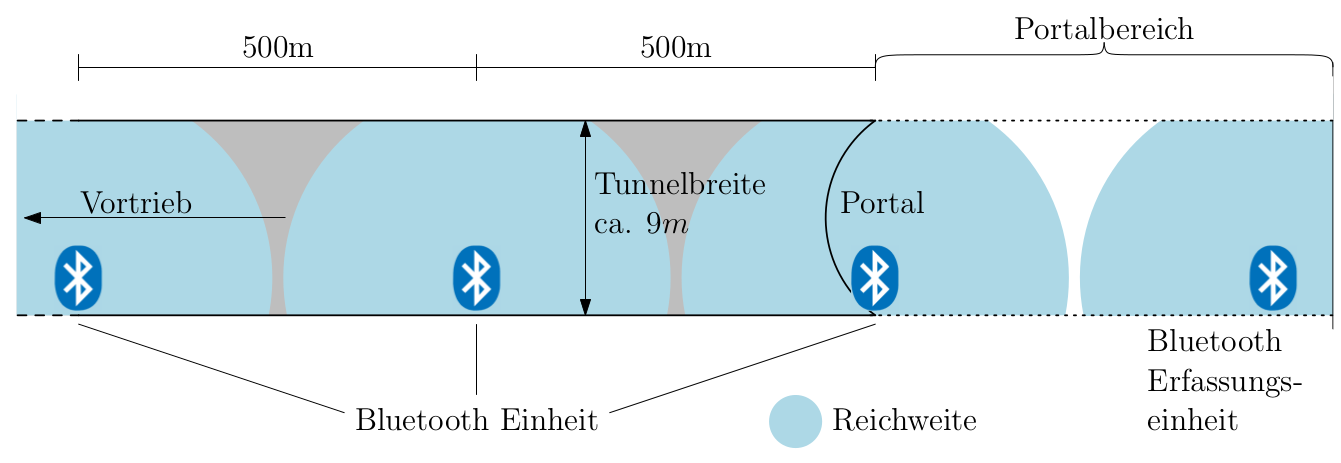
\includegraphics[width=\textwidth]{images/bisherige.png}
  \caption{Bereichsortung mit Bluetooth, aus \cite{maurer2016unterstuetzung}.}
  \label{fig:bisherige}
\end{figure}

 
\section{Umgebung für funkbasierte Ortung}
Als Versuchsumgebung dient die Tunnelbaustelle Rastatt.
Dort gelten die Positionen der Kästen für die Technik als unveränderlich.
Nur sie bieten Strom, Netzwerkanbindung (LAN) und Schutz vor dem Baustellenumfeld.
Für Funkprotokolle, die weniger als 250 Meter Reichweite entfalten muss daher mit Erfasssungslücken gerechnet werden.
Auf der TBM und anderen technischen Fahrzeugen sind jedoch mehr Basisstationen möglich.

Es existiert bereits ein WLAN-Netzwerk, dessen Access Points als Basisstationen genutzt werden können.
Es handelt sich um APs der Firma Lancom, diese stellt auch ein Modell LN-862 für Versuche.
Für zukünftige Baustellen soll der Abstand der Versorgungskästen auf 250 Meter sinken. 
Diese Situation ist in Abbildung \ref{fig:zukuenftige} skizziert.

\begin{figure}[h]
  \centering
	\includegraphics[width=\textwidth]{images/zukuenftige.eps}
  \caption{Zukünftige Situation der Tunnelbaustellen.}
  \label{fig:zukuenftige}
\end{figure}

\section{Problemstellung}
Es muss ein System geschaffen werden, welches Mitarbeiter einem 250 Meter langen Abschnitt innerhalb eines im Bau befindlichen Tunnels zuordnet.
Dazu soll keine Nutzerinteraktion nötig sein, der Nutzer wird wird über eine mobile Einheit geortet.
Die Ortung muss unterirdisch funktionieren und robust gegenüber Stahlhindernissen sein.
Außerdem können Basisstation für die Ortung nur alle 250 Meter platziert werden.


\section{Zielsetzung der Arbeit}
\label{ch:Einleitung:sec:Zielsetzung}
Ziel der Arbeit soll der Entwurf und die Implementierung eines Bereichsortungssystems für Personen in Tunnelanlagen sein. 
Bei einem Bereichsortungssystem handelt es sich um ein Ortungssystem, bei dem die Positionen nicht genau bestimmt werden. 
Stattdessen wird das Areal, auf dem geortet werden soll, in einzelne Bereiche unterteilt und jede mobile Einheit beim Vorgang des Ortens einem dieser Bereiche zugeordnet.

Diese Arbeit grenzt sich von vorherigen Arbeiten dadurch ab, dass die Laufzeit beziehungsweise der Energieverbrauch der mobilen Einheiten im Vordergrund steht. 
Ziel dieser Arbeit ist eine mehrmonatige Laufzeit der mobilen Einheiten. 

Für diese Arbeit werden mehrere Prototypen für mobile Einheiten entwickelt und auf ihre Charakteristik bezüglich des Energieverbrauchs und der Erkennungszuverlässigkeit untersucht.
Der Entwurfsraum umfasst dabei die Hardware und Software der mobilen Enheit sowie die Implementierung des Ortungsdienstes. 
Die für die Funktechnologie benötigte Infrastruktur wird jeweils als gegeben angenommen.


\section{Anforderungen an das Bereichsortungssystem}
\label{ch:Einleitung:sec:Anforderungen}
Da es sich um ein Bereichsortungssystem handeln soll, werden keine direkten Anforderungen an die Genauigkeit der Ortung gestellt. 
Jedoch soll ein klarer Wechsel zwischen zwei Bereichen, und damit zwei Basisstationen, zuverlässig erkannt werden. 
Die mobilen Einheiten sollen von Personen um den Hals getragen werden können. 
Dies bedingt ein geringes Gewicht des Akkus, gleichzeitig soll aber die Laufzeit der mobilen Einheit maximiert werden, sodass ein Akku mit möglichst großer Kapazität gewählt werden sollte.
Zuletzt soll unter Rücksichtnahme auf das beschriebene Szenario die Komplexität der benötigten IT-Infrastruktur so gering wie möglich gehalten werden um ein stabiles und kostengünstiges System zu garantieren. 


\section{Gliederung der Arbeit}
\label{ch:Einleitung:sec:Gliederung}
Nachdem zunächst in Kapitel \ref{ch:Grundlagen} die Grundlagen der funkbasierten Ortung und der verwendeten Funkprotokolle behandelt werden, wird in Kapitel \ref{ch:Analyse} das Problem analysiert und verwandte Arbeiten aufgezeigt.
Kapitel \ref{ch:Implementierung} beschäftigt sich mit der Implementierung und Untersuchung der Prototypen. 
Das Fazit in Kapitel \ref{ch:Fazit} fasst die Arbeit noch einmal zusammen, vergleicht und bewertet die Ergebnisse.
  % Einleitung
\chapter{Phase 1 - Keine Veränderungen an den APs}
\label{ch:phase1}
In einem ersten Schritt sollten laut Aufgabenstellung keine Veränderungen an den Access Points vorgenommen werden können.
Weil die Ortung deshalb auf WLAN basieren muss sind die Knoten im Folgenden immer APs. 
Ein Tag ist eine mobile Einheit, umgekehrt gilt dies jedoch nicht, da auch alle anderen WLAN-fähigen Geräte, wie Smartphones und Laptops, eine mobile Einheit sein kommen. \\
Die Unveränderlichkeit bedeutet insbesondere auch, dass keine Messwerte verwendet werden können, die direkt am AP gemessen werden müssen und nicht als Teil der 802.11 in das dahinterliegende Netzwerk weitergeleitet werden.
Da time of arrival Synchronisation und präzise Timer bei den APs vorraussetzt und time difference of arrival nur von den APs gemessen werden kann, eignen sich diese Messgrößen nicht für diese Aufgabenstellung.
Received signal strength und roundtrip time of flight können auf der mobilen Einheit gemessen werden, nicht jedoch an den APs, da die in der PHY- beziehungsweise MAC-Schicht gemessenen Werte nicht an weitere Empfänger im Netzwerk propagiert werden. 
Somit scheidet die direkte Fernlokalisierung mangels Messgrößen aus, es wird stattdessen eine indirekte Fernlokalisierung durchgeführt bei der die mobile Einheit eine Selbstlokalisierung durchführt und das Ergebnis dem Ortungsserver über eine Datenverbindung mitteilt.


\section{Vorherige Arbeiten}
\label{ch:phase1:sec:vorherige}
Zunächst werden vorherige Arbeiten behandelt, es werden sowohl wissenschaftliche als auch kommerzielle Lösungen betrachtet.


\subsection{WiFi-LLS}
\label{ch:Vorherige:sec:LLS}
Chen et al. stellen mit dem WiFi-based Local Location System (WiFi-LLS) ein System zur indirekten Fernlokalisierung vor \cite{chen2007design}.
Als Messgröße wird die Stärke des empfangenen Signals (received signal strength, RSS) genutzt, diese wird laut 802.11 Spezifikation als Index (RSSI) von der Hardware zurückgegeben. \\
Für die Ortung wird zunächst der RSSI von Paketen naher APs gemessen und zusammen mit der MAC-Adresse der mobilen Einheit in ein Paket gepackt und an den Ortungsserver versendet.
Anschließend wird auf dem Ortungsserver ein theoretisches Signalausbreitungsmodell $P(d) = P(d_0) - 10log_{10}(\frac{d}{d_0})^n - OAF$ mit der Distanz $d$, der Signalstärke $P(d)$ und der Referenzdistanz $d_0 = 1m$ zur Bestimmung der Position der mobilen Einheit verwendet. \\
$P(d_0)$, der Pfadverlustexponent $n$ und der Hindernisdämpfungsfaktor $OAF$ müssen bestimmt werden, jedoch lassen sich $P(d_0)$ und $n$ auf einer einzelnen Teststrecke mit unterschiedlichen Abständen von AP und mobiler Einheit bestimmen. $OAF$ kann sogar für einen Gebäudetyp einmalig bestimmt werden.
Dadurch hat das Modell einen konstanten Aufwand. 
Dies ist für Baustellen interessant, da sich diese Werte einmalig messen und dann sogar über mehrere gleichartige Baustellen übertragen ließen.\\
In dieser Veröffentlichung steht die Ortungsgenauigkeit im Vordergrund und es werden keine Angaben zum Energieverbrauch gemacht. 
Als Referenz kann dienen, dass die mobile Einheit bei WiFi-LLS alle 5 Sekunden einen Scan (siehe Abschnitt \ref{ch:phase1:sec:scan}) durchführt, dann werden die Signalstärken entdeckten APs zusammen mit der eigenen MAC-Adresse in XML codiert und das so erzeugte Paket an den Ortungsserver versendet.

\subsection{AiRISTA Flow RTLS}
Ekahau bietet unter der Marke \textit{AiRISTA Flow RTLS} eine, zu WiFi-LLS ähnliche, Lösung kommerziell an \cite{airista2017airista}.
Ihr Ekahau B4 Badge Tag ermittelt regelmäßig den RSSI zu nahegelegenen Access Points und versendet diese an einen Ortungsserver \cite{liu2007survey}.
Das Tag bietet darüber hinaus noch einige Zusatzfunktionen, so können über die Datenverbindung auch Nachrichten und Alarmierungen an das Tag gesendet werden und die drei angebrachten Knöpfe können programmiert werden.\\
Bezüglich des Energieverbrauchs gibt sich das Informationsblatt des B4 Badge Tag vage: Das Tag soll abhängig vom Ortungsintervall wochenlang halten, danach muss der $600\ mA/h$ Akku geladen werden \cite{ekahau2017b4}.
Das Informationsblatt zum Ekahau W4, welches statt um den Hals am Handgelenk getragen wird, gibt an, dass der verbaute $530\ mA/h$ Akku bei einem Ortungsintervall von 15 Sekunden 500 Stunden (ca. 21 Tage) hält \cite{ekahau2017w4}.\\
AiRISTA Flow spricht auf ihrer Website zum Beispiel Krankenhäuser, Schulen und Regierungseinrichtungen an, hier sollen zusätzlich bewegliche Objekte, wie etwa Krankenhausbetten, geortet werden.
Die dazu verwendeten Asset Tags werden über einen Beschleunigungssensor aktiviert und können, wenn die Objekte selten bewegt werden, deutlich längere Laufzeiten erreichen \cite{ekahau2017a4}. \\

\subsection{AeroScout}
Auch das AeroScout System von Stanley Healthcare richtet sich an den medizinischen Sektor und soll Objekte und Personen orten \cite{aeroscout2017asset}, \cite{aeroscout2017staff}.
Da sich auch dieses System in das bestehende WLAN-Netzwerk einfügt, sollte es ebenfalls auf einer indirekten Fernlokalisierung beruhen und demnach ähnliche Eigenschaften bezüglich des Energieverbrauchs aufweisen.\\
Das Informationsblatt ihres T14 Tags für Personen gibt eine Laufzeit von bis zu drei Wochen, abhängig von Konfiguration und Typ des Tags, an \cite{aeroscout2017t14}. 
Eine Angabe zu dem verwendeten Typ, der Konfiguration oder der Kapazität des verbauten Akkus wird nicht gemacht.\\

\subsection{Selbstlokalisierung mit Szenenanalyse}
\label{ch:Vorherige:sec:RSS-basierte}
Prasithsangaree et al. stellen ein System zur Selbstlokalisierung vor \cite{prasithsangaree2002indoor}, es verwendet aber eine offline-Phase zum Sammeln von Fingerabdrücken für Positionen in einem Abstand von 1,5 beziehungsweise 3 Metern. 
In diesen Fingerabdrücken werden die gemessenen RSSI der von den APs empfangenen Pakete als Merkmale zusammen mit der Position als Label gespeichert.
In der anschließenden online-Phase werden die gemessenen RSSI mit den Fingerabdrücken verglichen und die Position als gewichtetes Mittel der Labels bestimmt. \\
Die offline-Phase ist natürlich im Sinne der Aufgabenstellung nicht sinnvoll, da für eine Tunnelbreite von 10m 4000 beziehungsweise 2000 Messungen pro Kilometer vorgenommen werden müssten.
Generell eignen sich Lösungen mit Szenenanalyse nicht gut für Baustellen, da diese nicht auf die potentiell höhere Genauigkeit angewiesen sind. 
Üblicherweise müssen dort sehr große Flächen vermessen werden und die Veränderungen durch den Baufortschritt führen dazu, dass regelmäßig neu gemessen werden muss.
Außerdem müssen bewegliche Störquellen wie Baumaschinen vorher aus dem Bereich entfernt werden, um unverfälschte Fingerabdrücke zu erhalten.
Der Aufwand ein System mit Szenenanalyse auf einer Baustelle zu betreiben ist deshalb sehr hoch und widerspricht der Forderung nach geringer Komplexität. \\
Die Arbeit zeigt aber die Volatilität der empfangenen Signalstärke auf, dies wurde 2011 von Lui et al. genauer untersucht \cite{lui2011differences}.
Lui et al. zeigen, dass die gemessene empfangene Signalstärke stark von der beteiligten Hardware abhängt und die Systeme jedes mal neu kalibriert werden müssen wenn sie auf ein neues AP-Modell portiert werden. 
Auf dem Areal sollte deshalb optimalerweise nur ein AP-Modell verwendet werden. \\
Abb. \ref{fig:luiRSSI} zeigt die gemessenen RSSI Werte für die von ihnen getesten Netzwerkkarten mit unterschiedlichen Distanzen, für einige Karten korreliert die empfangene Signalstärke nur sehr schwach mit der Distanz zwischen Knoten und mobiler Einheit.
Sie zeigen außerdem, dass einige AP-Modelle den RSSI speichern und nur bei größeren Veränderungen aktualisieren und dass die Antenne signifikanten Einfluss auf den protokollierten Wert hat.



\begin{figure}[h]
  \centering
	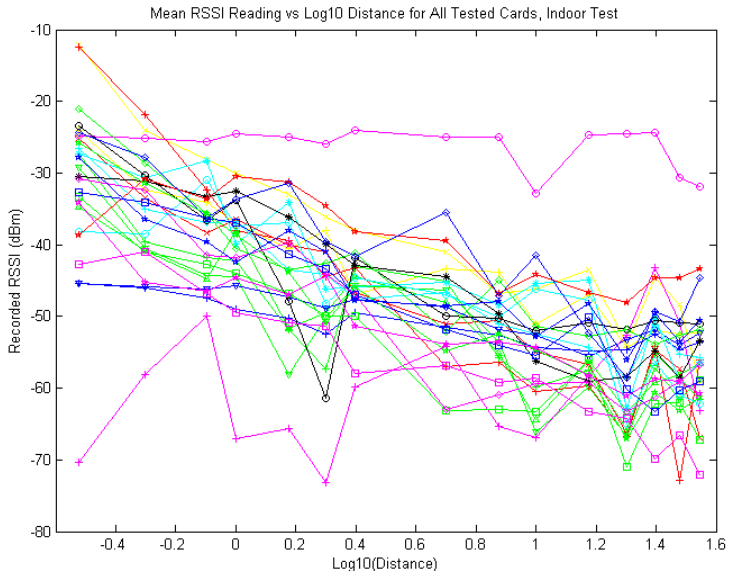
\includegraphics[width=\textwidth]{images/luiRSSI.png}
  \caption{Gemessener RSSI mit verschiedenen Access Points und Distanzen, aus \cite{lui2011differences}.}
  \label{fig:luiRSSI}
\end{figure}

\section{Grundlagen der 802.11 Spezifikation}
\label{ch:phase1:sec:grundlagen}
802.11 beschreibt eine Form der drahtlosen Datenübertragung mittels Funkwellen \cite{ieee2012macphy}.
Die Spezifikation beschreibt die physische Schicht (PHY-Layer) und den Mediumszugriff (MAC-Layer) für ein Funknetzwerk, dass sich mit den darüber liegenden Schichten des OSI-Modells in andere Netzwerke eingebunden werden kann.
Wird ein solches Netzwerk in ein Local Area Network (LAN) eingebunden spricht man üblicherweise vom Wireless Local Area Network (WLAN).
Die 1997 erstmals verabschiedete Spezifikation wurde häufig erweitert und wird in ihrer ursprünglichen Form praktisch nicht mehr angewendet, da die Datenraten zu gering sind.
Die Erweiterungen werden mit Buchstaben benannt (zum Beispiel 802.11g) und verändern entwa die verwendete Frequenz und Modulationsverfahren.\\
Zur Vermeidung von Kollisionen kommt Carrier Sense Multiple Access/Collision Avoidance (CSMA/CA) zum Einsatz.
Bei CSMA/CA wird zunächst das Medium belauscht und gewartet bis keine Signale mehr auf dem Medium sind. 
Dann muss ein Inter Frame Spacing (IFS) abgewartet werden, je nach Priorität ist dieses unterschiedlich lang (SIFS<PIFS<DIFS<EIFS), anschließend kann gesendet werden.
Tritt trotzdem eine Kollision auf, versucht der Sender es erneut mit einem längeren IFS.\\
802.11 spezifiziert ebenfalls mehrere Operationen, die beispielsweise zur Entdeckung von Ressourcen und der Authentifizierung an einer Ressource dienen, einige, für diese Arbeit wichtige Operationen werden im Folgenden beschrieben.

\subsection{Scan}
\label{ch:phase1:sec:scan}
Scan ist eine Operation zur Entdeckung von Access Points, sie kann von einer Station (Endverbraucher, zum Beispiel Smartphone oder Laptop) aktiv oder passiv ausgeführt werden \cite{ieee2012scan}.
Bei einem passiven Scan empfängt die Station und filtert die von Access Points regelmäßig gesendeten Beacons heraus, diese gelten dann als entdeckt.
Ein Beacon Frame ist ein Management Frame, der dazu gedacht ist, technische Möglichkeiten des APs zu bewerben, zum Beispiel die möglichen Datenraten und Zeitstempel zur Synchronisierung.
Versteckte APs senden keine Beacons. \\
Bei einem aktiven Scan sendet die Station einen Probe Request aus, dieser kann sowohl an alle APs (broadcast) als auch an einen speziellen AP adressiert sein.
Ein Probe Requests bewirbt, ähnlich wie ein Beacon, die technischen Möglichkeiten der Station.
Der addressierte AP, beziehungsweise im Falle des broadcasts alle APs, beantwortet den Probe Request mit einer Probe Response in der er mitteilt welche der beworbenen Funktionen er ebenfalls unterstützt, die Station schließt den Vorgang mit einem Acknowlegement ab. \\
Das 2,4GHz ISM-Band wird in Europa in 13 je 10MHz breite Kanäle aufgeteilt, da ein AP immer nur auf einem Kanal aktiv ist müsste jeder Kanal gescannt werden.
Praktisch werden jedoch breitere Kanäle verwendet, 802.11g verwendet beispielsweise 20MHz breite Kanäle, so dass effektiv nur die Kanäle 1, 5, 9 und 13 geprüft werden müssen. \\
Tabelle \ref{table:management} listet alle in der 802.11 Spezifikation gelisteten Management Frames.
Ein Management Frame wird durch die Typenbits markiert und durch die Bits für den Subtypen weiter unterschieden.

\begin{table}[h]
	\centering
	\caption{Management Frames nach 802.11 \cite{ieee2012management}}
	\label{table:management}
	\begin{tabular}{l|l|l}
		Type & Subtype & Beschreibung \\
		\hline
		00 & 0000 & Association Request  \\
		00 & 0001 & Association Response  \\
		00 & 0010 & Reassociation Request  \\
		00 & 0011 & Reassociation Response  \\
		00 & 0100 & Probe Request  \\
		00 & 0101 & Probe Response  \\
		00 & 0110 & Timing Advertisement  \\
		00 & 0111 & Reserved  \\
		00 & 1000 & Beacon  \\
		00 & 1001 & ATIM  \\
		00 & 1010 & Disassociation  \\
		00 & 1011 & Authentification  \\
		00 & 1100 & Deauthentification  \\
		00 & 1101 & Action  \\
		00 & 1110 & Action No Ack  \\
		00 & 1111 & Reserved  \\
	\end{tabular}
\end{table}

\subsection{Join}
Aus den entdeckten APs kann nun einer ausgewählt werden um seinem Netzwerk (BSS) beizutreten \cite{ieee2012join}.
Es kann zwar geschehen, dass mehrere APs eines Netzwerks entdeckt wurden, eine Statíon kann jedoch zu jedem Zeitpunkt nur mit einem AP assoziert sein. \\
Um einem Netzwerk beizutreten muss sich die Station zunächst authentifizieren, dieser Vorgang wird über einen Authentication Frame (siehe Tabelle \ref{table:management}) initiiert \cite{ieee2012auth}. 
Das weitere Vorgehen hängt vom Authentifizierungsverfahren ab, zum Beispiel kann der AP einen verschlüsselten Challenge Text an die Station senden, der mit einem aus dem Passwort erzeugten Schlüssel entschlüsselt wird und an den AP zurück gesendet werden kann. 
Ist die Antwort korrekt bestätigt der AP den Vorgang mit einem Acknowledgement und eventuell zusätzlichen Informationen für eine Stromchiffre. \\
Anschließend kann die Station mit dem AP assoziiert werden \cite{ieee2012associate}. 
Sie erhält nun eine IP und der AP gibt dem Netzwerk bekannt, dass er für die Station zuständig ist, dies geschiet  üblicherweise über das Address Resolution Protokoll (ARP). [evtl IGMP?] \\
Ist eine Station assoziert kann sie Datenverbindungen mit anderen Teilnehmern im Netzwerk aufbauen, sie könnte beispielweise das HTTP-Protokoll nutzen um eine Webseite anzufordern.

\subsection{Reassociation}
Eine Reassociation wird durchgeführt wenn die Station keine gute Verbindung mehr zu ihrem AP hat und ein AP des selben Netzwerks verfügbar ist, der eine bessere Verbindung bietet \cite{ieee2012reassociate}.
Um diesen neuen AP zu entdecken muss zunächst ein Scan durchgeführt werden. \\
Anschließend sendet die Station einen Reassociation Request an den neuen AP, im Reassociation Request wird der alte AP benannt, so dass der neue AP überprüfen kann, ob die Station tatsächlich mit ihm assoziert ist, gepufferte Pakete von ihm entgegennehmen und die Assoziation mit ihm auflösen kann.
Der Kommunikationsvorgang zwischen den APs wird auch als Handoff bezeichnet, wird dieser erfolgreich abgeschlossen antwortet der neue AP der Station mit einer Reassiciation Response.
Abschließend wird dem Netzwerk die neue Assoziation mittels ARP mitgeteilt.

\begin{figure}[h]
  \centering
	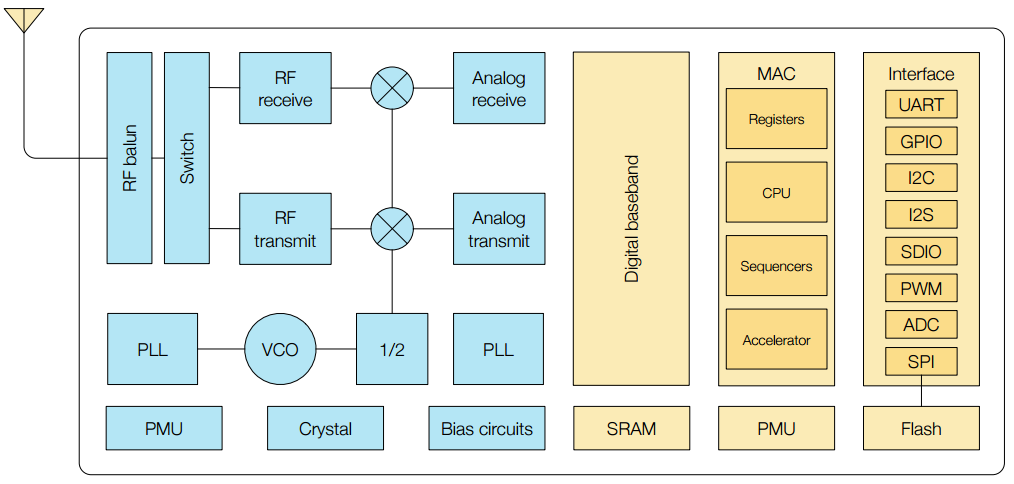
\includegraphics[width=\textwidth]{images/espblock.png}
  \caption{Blockdiagramm des ESP8266, aus \cite{espressif2017esp8266}}
  \label{fig:espblock}
\end{figure}

\section{ESP8266}
Der ESP8266 soll als Hardware für das Tag eingesetzt werden, dabei handelt es sich um einen Microcontroller von Espressif.
Der Esp8266 besitzt neben einer CPU eine 802.11b/g/n"-/e/i-fähige WLAN-Einheit und diverse andere, kabelgebundene Kommunikationsstandards wie zum Beispiel GPIO, I2C und SPI, siehe Abb. \ref{fig:espblock}. \\
Da der ESP8266 selbst weder über Flashspeicher, noch über eine Antenne verfügt wird er auf einem Modul mit diesen Komponenten verbaut, die in dieser Arbeit betrachteten Module sind das ESP12-S und das ESP12-F.
Das neuere ESP12-F sollte eine höhere Reichweite bei der Funkübertragung entfalten, dies wird noch Gegenstand eines Experiments sein.
Abb. \ref{fig:espmodules} zeigt die beiden Module nebeneinander, die unterschiedlichen Antennenformen sind deutlich zu erkennen.\\
Espressif gibt im Datenblatt auch Aufschluss über den Energieverbrauch des ESPs, siehe dazu Abb. \ref{fig:esppower}.
Für die Prototypenentwicklung wird ein ESP12-S Modul auf einem Adafruit Feather Huzzah verwendet, dieses stellt mit dem CP2104 eine serielle Schnittstelle zum ESP her, reguliert die Spannung für das Modul auf 3,3V und bringt den 2mm Pinabstand des ESP12-S Moduls auf die für Breadboards üblichen 2,5mm.
Das Adafruit Feather Huzzah mit ESP12-S ist in Abb. \ref{fig:espmodules} links abgebildet.

\begin{figure}[h]
  \centering
	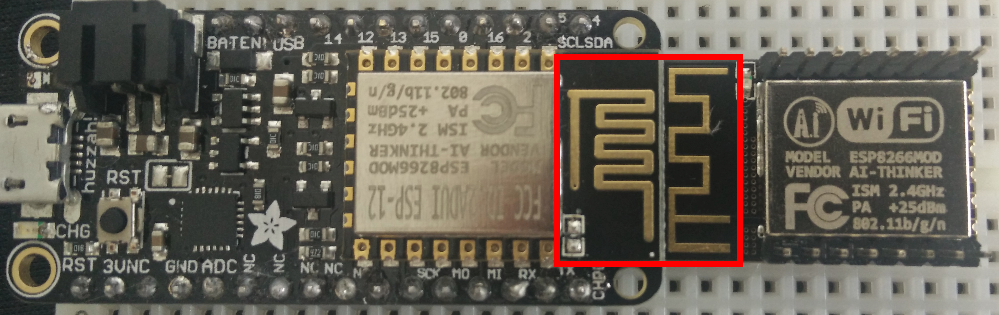
\includegraphics[width=\textwidth]{images/espmodules.png}
  \caption{Vergleich der Antennen, links: ESP12-S verbaut auf einem Adafruit Feather Huzzah, rechts: ESP12-F}
  \label{fig:espmodules}
\end{figure}

\begin{figure}[h]
  \centering
	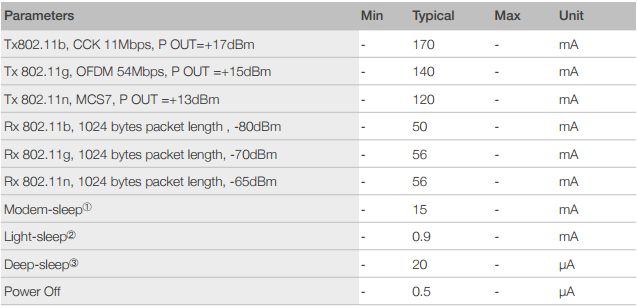
\includegraphics[width=\textwidth]{images/esppower.png}
  \caption{Energieverbrauch des ESP8266 bei verschiedenen Operationen, aus \cite{espressif2017esp8266}}
  \label{fig:esppower}
\end{figure}


\subsection{ESP8266 Arduino Core}
Eine einfache Möglichkeit den ESP8266 zu programmieren stellt die bekannte Arduino IDE dar \cite{banzi2017arduino}.\\
Unter Windows muss zunächst der Treiber für den \textit{CP2104 USB-to-Serial Chip} installiert werden, auf Linux und Mac entfällt dieser Schritt \cite{fried2017feather}.
Nach der Installation der Arduino IDE muss dort in den Einstellungen unter \textit{Additional Boards Manager URLs} die URL \url{http://arduino.esp8266.com/stable/package_esp8266com_index.json} hinzugefügt werden.  
Nach einem Neustart der IDE kann im \textit{Boards Manager} das Paket für den ESP8266 heruntergeladen werden und anschließend das Board \textit{Adafruit HUZZAH ESP8266} ausgewählt werden. \\
Ist das Board über USB mit dem Computer verbunden kann nun eigener Code oder eines der Beispiele aus \textit{Examples for Adafruit HUZZAH ESP8266} mit STRG+U auf den ESP geladen werden. 
Dieser Vorgang wird im Folgenden als flashen bezeichnet. \\
Der ESP8266 Arduino Core wird als Open Source Projekt gepflegt und setzt die ESP Open SDK auf einen, für die Arduino IDE üblichen Stil um \cite{arduino2017core}. 
Dabei wird möglichst die Kompatibilität zu Arduino gewahrt, das führt oft dazu, dass bereitgestellte Funktionen der SDK nicht in Arduino umgesetzt wurden.
Sollten die Funktionen dennoch benötigt werden können die Header-Dateien der SDK direkt importiert werden:

\begin{verbatim}
//Hier wird ein Header des ESP8266 Arduino Core importiert
#include <ESP8266WiFi.h> 

//Hier wird ein Header der ESP Open SDK importiert
extern "C" {#include "user_interface.h"} 
\end{verbatim}

Der ESP8266 Arduino Core wurde in der Version 2.3.0 verwendet.

\subsection{ESP Open SDK}
Statt mit der Arduino Core Umsetzung der ESP Open SDK kann natürlich auch direkt mit ihr programmiert werden \cite{esp2017open}. \\
Dazu muss zunächst das Github Projekt geklont werden: \texttt{git clone --recursive \url{https://github.com/pfalcon/esp-open-sdk}.git} und anschließend mit \texttt{make} kompiliert werden.
Wurde die Kompilierung erfolgreich abgeschlossen sollte die Pfadvariable (PATH) entsprechend der Meldung des make-Tools erweitert werden. \\
Die in C geschriebenen Programme können nun mit einem modifizierten GCC-Kompiler kompiliert und anschließend mit dem esptool.py zunächst in ein Image umgewandelt und dann geflasht werden. 
Das in \textit{examples} enthaltene \textit{blinky} Beispiel beinhaltet neben dem Beispielcode eine Makefile, in der diese Schritte nachvollzogen werden können, mit \texttt{make flash} wird das Beispiel kompiliert und geflasht. \\
Programme werden in regulärem C unter Zuhilfenahme der in \texttt{/sdk/include} enthaltenen Header-Dateien geschrieben, zu beachten ist nur, dass einige Funktionen der \texttt{stdlib.h} nicht verwendet werden können.
Dies betrifft vor allem direkten Speicherzugriff wie zum Beispiel \texttt{memcpy}, hier muss stattdessen \texttt{os\_memcpy} verwendet werden.
Alle betroffenen Funktionen sind in \texttt{osapi.h} beschrieben. \\
Einige frühe Experimente zeigten, dass Programme, die mit der ESP Open SDK geschrieben wurden auf dem ESP schneller starten als solche, die mit dem ESP8266 Arduino Core geschrieben wurden.
Diese Andeutung von Ineffizienzen bei der Übersetzung von Arduino Code wurde zum Anlass genommen, für die nachfolgenden Implementierungen nach der Fertigstellung des Prototypen in Arduino ebenfalls eine Implementierung in C hinzuzufügen, um ein optimales Programm zu erhalten. \\
Die ESP Open SDK wurde in der Version 2.0.0 verwendet.



\section{WiFi-LSS Implementierung}
Die mobile Einheit des WiFi-LLS Systems führt alle 5 Sekunden einen Scan aus, kodiert die Ergebnisse in XML und versendet sie an den Ortungsserver \cite{chen2007design}.
Da der Fokus dieser Arbeit auf dem Energieverbrauch liegt werden für die Referenzimplementierung eines WiFi-LLS-Tags die Kodierung in XML durch eine simple String Kodierung ersetzt und die Ergebnisse werden über UDP an den Ortungsserver übermittelt. 
Damit wird der overhead einer TCP-Verbindung vermieden.\\
Zunächst muss sich das Tag dem Netzwerk beitreten (Join) und anschließend einen Scan ausführen und ein UDP-Paket versenden.
Da die Scan-Funktion des ESP8266 Arduino Core es nicht erlaubt den RSSI zu einem AP auszulesen muss \texttt{user\_interface.h} importiert und die Scan-Funktion der SDK direkt verwendet werden.
Um den Energieverbrauch weiter zu reduzieren, soll der ESP möglichst viel Zeit in Energiesparzuständen verbringen.
Der tiefste Schlafzustand, der dennoch eine Aufrechterhaltung der WLAN-Verbindung erlaubt ist der \texttt{light\_sleep}. 
Er wird vom ESP automatisch aufgerufen, wenn er keine Aufgaben zu erledigen hat.
Er kann aber auch manuell aufgerufen werden, beides wurde getestet.\\
Einige Parameter können gewählt werden: Insbesondere die Intervallzeit bestimmt, wie oft der ESP aktiv ist und damit auch wie viel Energie er verbraucht.
Für Mitarbeiter im Tunnel kann von einer Maximalgeschwindigkeit von $30\ km/h$ ausgegangen werden, diese wird durch Schienen- oder Lastkraftfahrzeuge erreicht. 
Die maximale Reichweite des ESP12-S beziehungsweise ESP12-F Moduls ist nicht bekannt und muss noch bestimmt werden, sie wird zwischen 50 und 100 Metern angenommen.
Es wurde daher ein Intervall von 5 Sekunden gewählt, in dieser Zeit bewegt sich ein Mitarbeiter bei $30\ km/h$ ca. $42\ m$.\\
Des Weiteren kann theoretisch die Zahl der gescannten Kanäle gewählt werden, da sich die Einflussbereiche der APs in einem WLAN-Netzwerk üblicherweise überlappen ist es aber sinnvoll diese über die 4 nichtüberlappenden Kanäle zu verteilen. 
Eine Implementierung die nur einen Kanal scannt tritt deshalb nur außer Konkurenz an.\\
Tabelle \ref{table:llsconsumption} zeigt den gemessen Energieverbrauch der Implementierungen in Arduino und C, jeweils mit und ohne manuell aufgerufenen \texttt{light\_sleep} und eine Implementierung, die nur einen Channel scannt.
Für die Tests wurde das Adafruit Feather Huzzah verwendet, es wurde mit $5\ V$ aus einer USB-Powerbank mit Energie versorgt, der Verbrauch wurde mit einem dazwischen geschalteten USB-Power-Meter gemessen.\\
Die Werte wurden stationär in einer Mietwohnung in einem 5-stöckigen Wohnhaus und damit nicht unter realen Bedingungen aufgezeichnet.
Unter realen Bedingungen finden durch die Bewegung des Mitarbeiters regelmäßig Reassizationen statt, im Gegenzug liefert ein Scan in einem Tunnel weniger Ergebnisse als in einem Wohnhaus.
Ein Test unter realen Bedingungen ist im Abschnitt \ref{kommtnoch} zu finden, er beinhaltet jedoch nur noch die Implementierung in C mit manuellem \texttt{light\_sleep} und einem Scan auf allen 4 Kanälen.

\begin{table}[h]
	\centering
	\caption{Energieverbrauch WiFi-LLS-artiger Tags}
	\label{table:llsconsumption}
	\begin{tabular}{p{3cm}|p{2.2cm}|p{1.5cm}|p{2cm}|p{2cm}|p{2cm}}
		SDK & manueller \texttt{light\_sleep} & Anzahl Kanäle & Spannung in V & $\varnothing$ Verbrauch in mA & $\varnothing$ Verbrauch in mW \\
		\hline
		Arduino Core & Nein & 4 & 5 & 22 & 110 \\
		Arduino Core & Ja & 4 & 5 & 21 & 105 \\
		ESP Open SDK & Nein & 4 & 5 & 19 & 95 \\
		ESP Open SDK & Ja & 4 & 5 & 19 & 95 \\
		\hline
		ESP Open SDK & Ja & 1 & 5 & 6,5 & 32,5 \\
	\end{tabular}
\end{table}

Die Tests zeigen, dass die Programmierung mit der ESP Open SDK einen Vorteil beim Energieverbrauch hat, dieser liegt bei ca $10\%$.
Andererseits fällt auf, dass die Reduzierung der gescannten Channel eine signifikante Senkung des Energieverbrauchs nach sich zieht, die Scan-Funktion ist also der Hauptverbraucher.\\
Um die finale Laufzeit zu bestimmen muss die Kapazität des Akkus bekannt sein.
Ein Lithium-Polymer Akku hat eine Nennspannung von $3,7\ V$, seine Kapazität wird in $mAh$ angegeben. 
Ein beispielhafter $1400\ mAh$ Lithium-Polymer Akku liefert folglich $1400\ mAh * 3,7\ V = 5180\ mWh$.
Die Laufzeit beträgt dann $5180\ mWh/95\ mW \approx 54,53\ h$, also etwas mehr als 2,25 Tage.

\section{Anpassungen für Bereichsortung}
\label{ch:phase1:sec:anpassungbereich}
Bei WiFi-LLS wird der Scan durchgeführt um den RSSI zu nahen Access Points zu erhalten und dann auf dem Ortungsserver die Position der mobilen Einheit mit einer Trilateration zu berechnen.
Im Tunnel sind oft nur ein bis zwei APs in Reichweite, außerdem wird eine Bereichsortung als ausreichend angesehen. \\
Werden die APs geschickt den Bereichen zugeordnet, reicht das Wissen um einen nahen AP um das Tag einem Bereich zuzuordnen.
Da dem Tag, welches im Sinne der 802.11 Spezifikation als Station arbeitet, die Adresse seines Netztzugangs (Gateway) bekannt sein muss, ist ihm die IP-Adresse des AP bekannt mit dem er assoziiert ist.
Diese Information wird nun als String kodiert und per UDP an den Ortungsserver versendet.\\
Tabelle \ref{table:naiveconsumption} zeigt den gemessen Verbrauch der Implementierungen in Arduino und C, jeweils mit und ohne manuell aufgerufenen \texttt{light\_sleep}.

\begin{table}[h]
	\centering
	\caption{Energieverbrauch der Bereichsortungstags}
	\label{table:naiveconsumption}
	\begin{tabular}{p{3cm}|p{2.2cm}|p{1.7cm}|p{2.5cm}|p{2.5cm}}
		SDK & manueller \texttt{light\_sleep} & Spannung in V & $\varnothing$ Verbrauch in mA & $\varnothing$ Verbrauch in mW \\
		\hline
		Arduino Core & Nein & 5 & 14 & 70 \\
		Arduino Core & Ja & 5 & 7 & 35 \\
		ESP Open SDK & Nein & 5 & 6 & 30 \\
		ESP Open SDK & Ja & 5 & 5,5 & 27,5 \\
	\end{tabular}
\end{table}

Der Verbrauch liegt wie erwartet unter dem der WiFi-LLS Implementierung, sogar unter der Implementierung, die nur einen Kanal scannt.
Wird der selbe $1400\ mAh$ beziehnungsweise $5180\ mWh$ Lithium-Polymer Akku angenommen liegt die Laufzeit diesmal  bei $5180\ mWh/27,5\ mW \approx 188,36\ h$, also bei fast 8 Tagen. \\
Als weitere Optimierung könnte ein Tag nur dann senden, wenn eine Reassoziation stattgefunden hat.
Die mangelnde Transportsicherheit von UDP macht dieses Vorgehen jedoch riskant, wenn das Paket verloren geht wird kein Bereichswechsel erkannt.
Um wieder eine begrenzte Transportsicherheit zu erhalten kann entweder das UDP-Paket mehrfach versandt werden; auch ohne Reassoziation in einen festen, aber größeren Intervall gesendet werden oder statt eine UDP-Verbindung eine TCP-Verbindung verwendet werden.
Somit ergeben sich neue Testszenarien: Ohne zusätzliche Sicherung, UDP-Paket mehrfach (dreifach) versenden, zusätzliches (30 beziehungsweise 60 Sekunden) Sendeintervall, TCP-Verbindung (offen halten oder nach dem senden schließen). \\
Da der Verbrauch nun stark von der Anzahl der Reassoziationen abhängt sind im gegeben, stationären Testszenario keine aussagekräftigen Ergebnisse möglich.
Dennoch sollen die Tests eine Ausgangswert ermitteln, dieser kann als untere Grenze für den Verbrauch einer Implementierung angesehen werden.
Da in den vorherigen Tests die Implementierungen mit der ESP Open SDK verbrauchsärmer waren, wurden alle in Tabelle \ref{table:naiveoptconsumption} gezeigten Implementierungen mit ihr erstellt, der manuelle \texttt{light\_sleep} ist immer aktiv.

\begin{table}[h]
	\centering
	\caption{Energieverbrauch der verbesserten Bereichsortungstags}
	\label{table:naiveoptconsumption}
	\begin{tabular}{p{3.5cm}|p{1.7cm}|p{2.5cm}|p{2.5cm}}
		Transportsicherung & Spannung in V & $\varnothing$ Verbrauch in mA & $\varnothing$ Verbrauch in mW \\
		\hline
		Ohne & 5 & 2 & 10 \\
		Dreifach UDP & 5 & 1,4 & 7 \\
		Zusatzintervall 30s & 5 & 2,62 & 13,1 \\
		Zusatzintervall 60s & 5 & 1,6 & 8 \\
		TCP (halten) & 5 & 1,2 & 6 \\
		TCP (schließen) & 5 & 1,07 & 5,35 \\
	\end{tabular}
\end{table}

Tests unter realen Bedingungen sind in Abschnitt \ref{kommtnoch} zu finden, dort wird xyz getestet.

[Mehr noch zur Tabelle]


\section{Direkte Fernlokalisierung mit IEEE 802.11}
\label{ch:phase2}
Bei der direkten Fernlokalisierung wird die Messgröße auf den Basisstationen gemessen.
Die Ortungsinformation wird dann implizit durch Versenden der gemessenen Werte an den Ortungsdienst übermittelt.
Dieser berechnet dann aus den gesammelten Werten die Position der mobilen Einheit.
Eine Lösung zur direkten Fernlokalisierung muss deshalb nicht mit einem \emph{Access Point} (AP) assoziiert sein.
APs versenden die gemessenen Werte jedoch nicht automatisch an den Ortungsdienst. 
Sollen also die APs des WLAN-Netzwerks auch als Basisstationen verwendet werden, muss ihre Software es erlauben den in der Analyse als Messgröße ausgewählten \emph{Received Signal Strength Indicator} (RSSI) bestimmter Pakete abzurufen.

%TODO Tags weg
\subsection{RADAR-Implementierung}
Eine mobile Einheit mit \emph{RADAR} versendet alle 0,25 Sekunden ein 6 Byte langes UDP-Paket, der RSSI der Übertragung wird dann auf dem AP gemessen.
Das Sende"-intervall wurde so kurz gewählt, um spontane Schwankungen im RSSI durch mehrfache Messung zu glätten und sich bewegende Personen möglichst genau zu erfassen.
Für eine Bereichsortung reicht ein wesentlich längeres Sendeintervall. 
Es wird erneut ein Intervall von 5 Sekunden gewählt, in dem sich ein Mitarbeiter maximal 42 m bewegt. 
Tabelle \ref{table:radarconsumption} zeigt den mit dem \emph{TM103} gemessenen Verbrauch der Implementierung für mobile Einheiten mit \emph{RADAR} jeweils in Arduino und C, mit unterschiedlich langen Sendeintervallen mit und ohne manuellem \texttt{light\_sleep}.

\begin{table}[h]
	\centering
	\caption{Stromverbrauch RADAR-artiger mobiler Einheiten}
	\label{table:radarconsumption}
	\begin{tabular}{l|p{2.2cm}|R{1.6cm}|R{2cm}|R{2cm}|R{2cm}}
		SDK & manueller \texttt{light\_sleep} & Sende"-intervall in Sekunden & Versuchs-dauer in Stunden & Gesamt"-verbrauch in mAh & $\varnothing$ Verbrauch in mA \\
		\hline
		Arduino Core & Nein & 0,25 & 2 & 80 & 40,00 \\
		Arduino Core & Ja & 0,25 & 3 & 119 & 39,66 \\
		Arduino Core & Nein & 5,00 & 3 & 28 & 9,33 \\
		Arduino Core & Ja & 5,00 & 3 & 23 & 7,66 \\
		ESP Open SDK & Nein & 0,25 & 1 & 40 & 40,00 \\
		ESP Open SDK & Ja & 0,25 & 1 & 38 & 38,00 \\
		ESP Open SDK & Nein & 5,00 & 2 & 12 & 6,00 \\
		ESP Open SDK & Ja & 5,00 & 2 & 10 & 5,00 \\
	\end{tabular}
\end{table}

Der Stromverbrauch einer Lösung die vier Pakete pro Sekunde sendet ist wie erwartet hoch.
Die Implementierungen mit der ESP Open SDK und manuellem \texttt{light\_sleep} unterscheiden sich ausschließlich im Sendeintervall, dies verändert den Stromverbrauch jedoch stark.
Die in Abschnitt \ref{ch:phase1:sec:anpassungbereich} besprochenen Optimierungen (Senden nur bei AP-Wechsel) können auch für die \emph{RADAR-Implementierung} verwendet werden, die \emph{RADAR}-artige mobile Einheit ist dann aber in seiner Implementierung bis auf den Inhalt des UDP-Pakets identisch mit dem der mobilen Einheiten für Bereichsortung.
Der Stromverbrauch sollte sich somit kaum unterscheiden und ein System mit \emph{RADAR}-artigen mobilen Einheiten benötigt Veränderungen der Software der APs, die \emph{Assoziations-Lokalisierung} ist deshalb vorzuziehen. 
Die Implementierung in C mit einem Sendeintervall von 5 Sekunden wird in Abschnitt \ref{ch:phase2:sec:powerradar} genauer untersucht.

\subsection{Probe-Request-Lokalisierung}
\label{ch:phase2:sec:anpassungbereich}
\emph{RADAR} versendet immer noch UDP-Pakete und arbeitet damit auf Schicht vier (Transport) des OSI-Modells. 
Die mobile Einheit muss im Netzwerk authentifiziert und mit einem \emph{Access Point} assoziiert sein.
Das ist für eine direkte Fernlokalisierung aber nicht notwendig, der RSSI wird auf Schicht eins (PHY) gemessen.
Grundsätzlich kann aufgrund der möglichen Änderungen am AP ein beliebiges Paket mit einer speziellen Kennung versendet und vom AP als Positionsmitteilung der mobilen Einheit erkannt werden. 

Ein Sendevorgang, der nur Schicht eins nutzt, hat einen geringeren Stromverbrauch, da er nur senden und nie empfangen muss.
Ein solcher Sendevorgang könnte aber die Funktion des Netzwerks beeinträchtigen und stellt nicht sicher, dass die eigene Übertragung nicht durch andere Übertragungen gestört wurde.
Außerdem kann der Entwickler oft nicht auf Schicht eins zugreifen, es sollte deshalb nicht auf Schicht eins gearbeitet werden.

Stattdessen sollte Schicht zwei (MAC) des OSI-Modells verwendet werden. 
Da IEEE 802.11 für den Mediumszugriff eine Kollisionsvermeidung (CSMA/CA) verwendet wird, muss die mobile Einheit vor dem Senden das Medium belauschen, um zu bestimmen ob es belegt ist.
Der Stromverbrauch ist somit pro Sendevorgang höher als bei einer Lösung auf Schicht eins, stellt dafür aber die Verfügbarkeit des Mediums (der Frequenz) für die übrigen Teilnehmer sicher. 

Um die Änderungen an der Software des AP gering zu halten, wurde der \emph{Probe Request} als zu sendender \emph{Frame} gewählt.
Es handelt sich dabei um einen \emph{Management Frame} (siehe Tabelle \ref{table:management}), der für den, in Abschnitt \ref{ch:phase1:sec:scan} beschriebenen, \emph{Scan}-Vorgang verwendet wird.
Der \emph{Probe Request} hat dabei den Vorteil, dass er bereits vom AP verarbeitet und mit einer \emph{Probe Response} beantwortet wird. 

Es wird also lediglich gefordert, dass der AP den Empfang des \emph{Probe Request} im Zuge der Verarbeitung protokolliert. 
Im Einzelnen müssen die Empfangszeit, der RSSI und die MAC-Adresse des Absenders protokolliert und für den Ortungsdienst abrufbar gemacht werden. 
Manche kommerziellen APs bieten ein solches Protokoll für \emph{Probe Requests} und \emph{Beacons} im Zuge einer \textit{Rogue Client/AP Detection} an \cite{lancom2017rouge}.

Die ESP Open SDK bietet über die Operationen wie \emph{Scan} und \emph{Join} hinaus mit \texttt{wifi\_send\_pkt\_freedom} eine Funktion zum Senden von Paketen auf Schicht zwei an.
Der \emph{ESP8266} Arduino Core implementiert diese Funktion nicht, stattdessen muss sie mit \texttt{extern \dq C\dq $\lbrace$\#include \dq user\_interface.h\dq $\rbrace$} importiert werden. 

\texttt{wifi\_send\_pkt\_freedom} setzt den PHY-Header selbst, der MAC-Header und Inhalt des Paketes müssen über einen Puffer übergeben werden.
\begin{verbatim}
uint8_t packet[26] = { 
/*0*/ 	0x40, //Version (2bit), Type (2bit), Subtype(4bit)
/*1*/ 	0x00, //Flags 
/*2*/ 	0x00, 0x00, //Duration
/*4*/   0xff, 0xff, 0xff, 0xff, 0xff, 0xff, //Destination MAC
/*10*/  0x01, 0x02, 0x03, 0x04, 0x05, 0x06, //Source MAC
/*16*/  0xff, 0xff, 0xff, 0xff, 0xff, 0xff, //BSSID, all ff=broadcast
/*22*/  0x00, 0x00, //Sequence Number (12bit), Fragment Number (4bit) 
//[End of MAC-Header][Start of Management tags]
/*24*/  0x83, //Tag Number (Path Reply 131) 
/*25*/ 	0x00, //Tag length
}; 
\end{verbatim}
Ein gewöhnlicher \emph{Probe Request} beinhaltet noch zusätzliche Informationen bezüglich seiner technischen Möglichenkeiten, wie etwa unterstützte Standards und Datenraten. 
Da die mobile Einheit aber nicht tatsächlich beitreten will, kann darauf verzichtet werden. 

Weil keine Verbindung mehr aufrecht erhalten werden muss, können tiefere Schlafzustände eingenommen werden. 
Statt des \texttt{light\_sleep} kann der \texttt{deep\_sleep} verwendet werden.
Dieser schaltet den \emph{ESP8266} und seinen Speicher fast vollständig ab, nach Ablauf der angegebenen Schlafzeit wird \emph{Pin 16} mit der Masse verbunden.
Damit der ESP wieder aufwacht, muss \emph{Pin 16} mit dem \emph{Reset Pin} (RST) verbunden werden, bei einem Reset initialisiert sich der \emph{ESP8266} neu.
Bei einer Lösung auf einer höheren Schicht würde dies dazu führen, dass die mobile Einheit versucht dem Netzwerk erneut beizutreten. 
Hingegen kann bei einer Lösung auf Schicht zwei sofort gesendet und danach wieder geschlafen werden.

Tabelle \ref{table:probeconsumption} zeigt den Stromverbrauch der Implementierungen jeweils mit manuell herbeigeführtem Schlafzustand, das Sendeintervall liegt bei konstant 5 Sekunden.

\begin{table}[h]
	\centering
	\caption{Stromverbrauch mobiler Einheiten mit Probe Request}
	\label{table:probeconsumption}
	\begin{tabular}{l|p{2.5cm}|R{2cm}|R{2cm}|R{2.5cm}}
		SDK & manueller Schlafzustand  & Versuchs-dauer in Stunden & Gesamt-verbrauch in mAh & $\varnothing$ Verbrauch in mA \\
		\hline
		Arduino Core & Ohne & 2 & 81 & 40,5 \\
		Arduino Core & light\_sleep & 2 & 10 & 5,00 \\
		Arduino Core & deep\_sleep & 4 & 17 & 4,25 \\
		ESP Open SDK & Ohne & 3 & 26 & 8,33 \\
		ESP Open SDK & light\_sleep & 25 & 75 & 3,00 \\
		ESP Open SDK & deep\_sleep & 48 & 39 & 0,81 \\
	\end{tabular}
\end{table}

%TODO Kann auch für genaue RSSI Trilateration genutzt werden.

Zu erkennen ist, dass die Verwendung des \texttt{deep\_sleep} zu einem geringeren Verbrauch führt. 
Allerdings benötigt die mit dem Arduino Core programmierte mobile Einheit im Vergleich zu der mit der ESP Open SDK programmierten Einheit deutlich länger zum Starten.
Sie verbraucht deshalb sogar mehr Strom als die mobilen Einheiten mit \emph{Assoziations-Lokalisierung} aus Abschnitt \ref{ch:phase1:sec:anpassungbereich}, die Implementierung mit der ESP Open SDK verbraucht aber weniger Strom als diese.
Hinzu kommt, dass sich der Verbrauch dieser mobilen Einheiten nicht durch die Bewegung des Trägers erhöht, da keine \emph{Reassoziationen} stattfinden.
Um die in Abschnitt \ref{ch:Einleitung:sec:Anforderungen} geforderten Laufzeiten zu erreichen, werden in Abschnitt \ref{ch:Beschleunigungssensor:sec:Abschaltautomatik} weitere Verbesserungen besprochen.
Die Implementierung in C mit \texttt{deep\_sleep} wird in Abschnitt \ref{ch:phase2:sec:powerprobereq} genauer untersucht.

\subsubsection{Anzahl der verwendeten Kanäle}
Eine Lösung, die nicht vor dem Versenden das Spektrum nach den APs durchsucht, muss entweder auf der Annahme beruhen, dass alle APs auf einem Kanal agieren oder auf allen in Frage kommenden Kanälen senden.

Je nach Erweiterung der 802.11 Spezifiktion ergeben sich unterschiedlich viele solcher Kanäle.
802.11b verwendet eine Kanalbreite von 22 MHz, es stehen daher effektiv nur drei Kanäle zur Verfügung: 1, 7 und 13 in Europa beziehungsweise 1, 6 und 11 in Nordamerika.
Für 802.11g/n mit 20 MHz Kanalbreite sind zwar in Europa theoretisch vier Kanäle verfügbar (1,5,9,13), es werden aber in der Praxis meist dieselben Kanäle wie bei 802.11b verwendet, um die Kompatibilität zu 802.11b zu gewährleisten.
802.11n ist auch für eine Kanalbreite von 40 MHz spezifiziert, hier stehen effektiv nur noch zwei Kanäle zur Verfügung. 
Üblicherweise werden Kanal 3 und 11 gewählt.

Die Implementierung in C mit \texttt{deep\_sleep} wurde sowohl auf einem, als auch auf drei Kanälen getestet.
Dabei ergab sich in 24 Stunden kein messbarer Unterschied.
Es sollte daher auf eine Festlegung des Kanals verzichtet werden, weil diese die reguläre Funktionsweise des WLAN-Netzwerks beeinträchtigen könnte.


\subsection{Untersuchung des Stromverbrauchs}
Erneut soll der Stromverbrauch mit dem INA219 genauer bestimmt werden, der INA219 und die verwendete Methodik werden in Abschnitt \ref{ch:phase1:sec:energie} beschrieben.


\subsubsection{RADAR}
\label{ch:phase2:sec:powerradar}
Abbildung \ref{fig:radar5s} zeigt den Lastverlauf nach dem Anschalten der mobilen Einheit für die Implementierung von \emph{RADAR}, wenn ein AP zur Verfügung steht. 
Der Beginn des Lastverlaufs ist dem der \emph{WiFi-LLS-Implementierung} ähnlich, es werden ebenfalls \emph{Scan} und \emph{Join} durchgeführt.

\begin{figure}[h!]
  \centering
	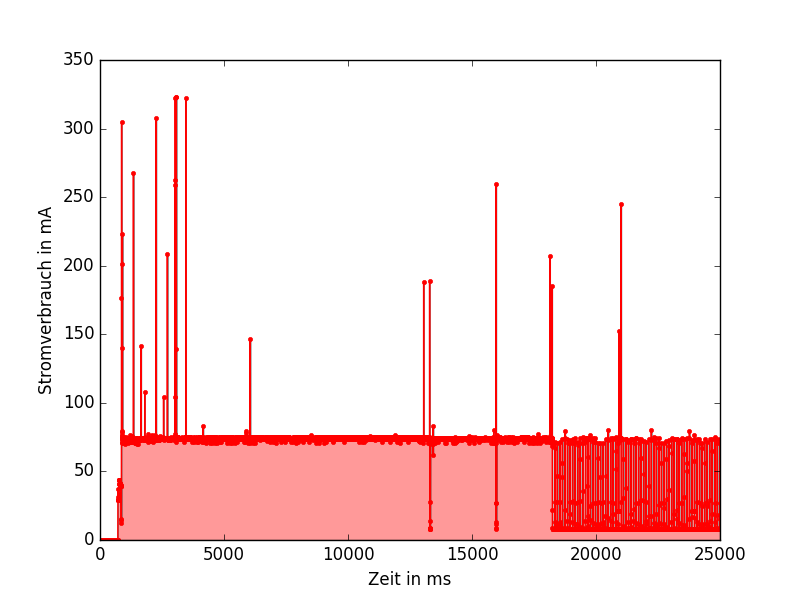
\includegraphics[width=\textwidth]{plots/radar5s.png}
  \caption{Stromverbrauchskurve einer Implementierung von \emph{RADAR}.}
  \label{fig:radar5s}
\end{figure}

Abbildung \ref{fig:radar5ssend} zeigt den Sendevorgang der \emph{RADAR-Implementierung}.
Auffällig ist, dass längerfristig empfangen wird, obwohl dies für den Versand des UDP-Pakets nicht notwendig ist.

\begin{figure}[h!]
  \centering
	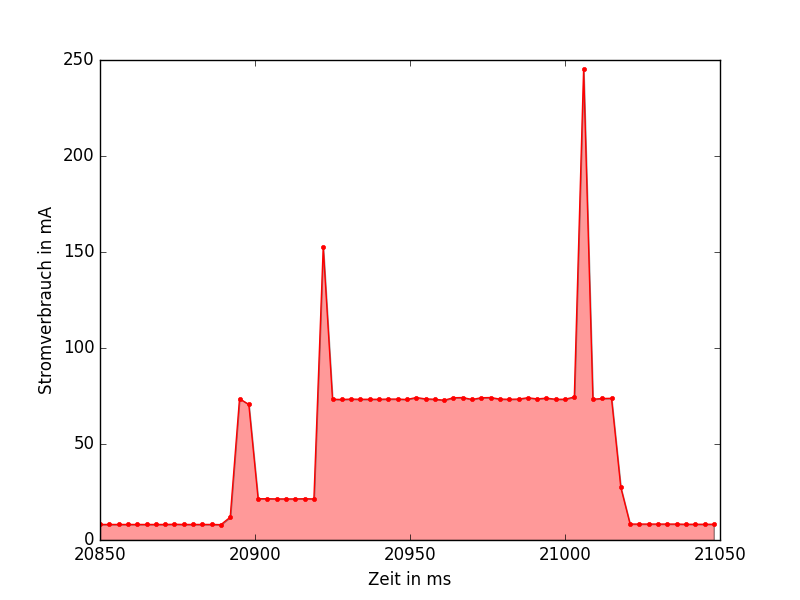
\includegraphics[width=\textwidth]{plots/radar5ssend.png}
  \caption{Stromverbrauchskurve eines Ortungsvorgangs mit RADAR.}
  \label{fig:radar5ssend}
\end{figure}

In Tabelle \ref{table:radarina} ist der durchschnittliche Verbrauch der \emph{RADAR}-Implementierung über eine Stunde gelistet.
Es wurde sowohl mit dem \emph{ESP8266} Feather, als auch mit dem einzelnen \emph{ESP-12F} gemessen, die mobile Einheit wurde jeweils erst circa eine Sekunde nach Beginn mit Strom versorgt.
Für den normalisierten Stromverbrauch wurde der Verbrauch im Ruhezustand subtrahiert. 
Dies beschränkt den Verbrauch auf den für die tatsächliche Funktion nötigen Anteil.

\begin{table}[h!]
	\centering
	\caption{Stromverbrauch mobiler Einheiten mit \emph{RADAR}-Implementierung}
	\label{table:radarina}
	\begin{tabular}{l|l|R{2.5cm}|R{2.5cm}}
		Hardware & Programm & $\varnothing$ Verbrauch in mA (normalisiert) & Laufzeit in Stunden\\
		\hline
		\emph{ESP8266} Feather & RADAR & 16,7 (8,6) & 83,8\\
		\emph{ESP-12F} & RADAR & 10,1 (8,8) & 138,6\\
	\end{tabular}
\end{table}

\subsubsection{Probe-Request-Lokalisierung}
\label{ch:phase2:sec:powerprobereq}
Abbildung \ref{fig:probereqfull} zeigt den Lastverlauf für eine mobile Einheit mit \emph{Probe-Request}-Implementierung und Abbildung \ref{fig:probereqv} zeigt den Lastverlauf für den Sendevorgang. 
Der Verlauf für den \emph{ESP8266} Feather ist in rot und der Verlauf für das \emph{ESP-12F} Moduls ist in grün dargestellt.

Nachdem der \emph{ESP8266} aus dem \texttt{deep\_sleep} erwacht, beginnt eine circa 100 Millisekunden andauerne Startphase, danach sendet er die drei \emph{Probe Requests}.
Anschließend soll der \emph{ESP8266} wieder in den \texttt{deep\_sleep} versetzt werden, vorher empfängt er jedoch noch 100 Millisekunden.
Die restliche Zeit befindet sich der \emph{ESP8266} im Tiefschlaf. 
Bei dem \emph{ESP-12F} Modul ist der INA219 nicht in der Lage einen Stromvebrauch zu messen, er liegt unter 0,1 mA.

\begin{figure}[h!]
  \centering
	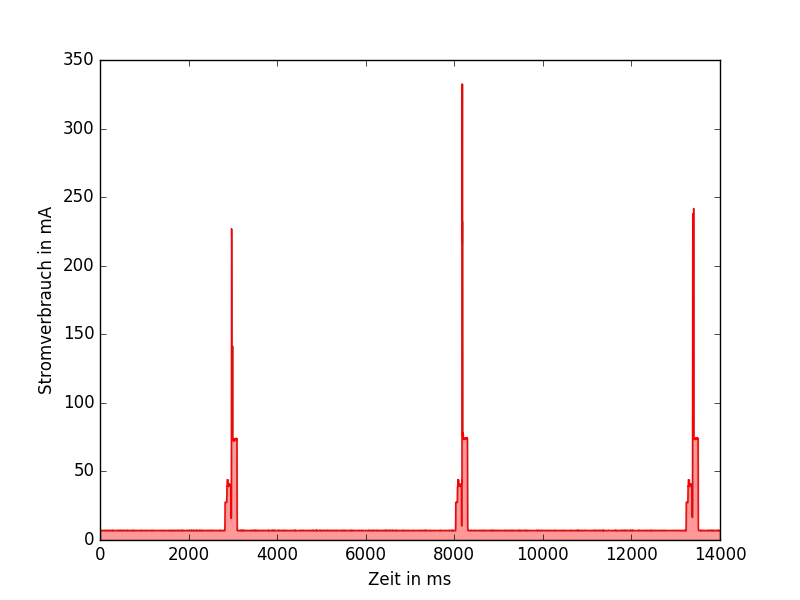
\includegraphics[width=\textwidth]{plots/probereqfull.png}
  \caption{Stromverbrauchskurve einer Implementierung mit \emph{Probe Requests}.}
  \label{fig:probereqfull}
\end{figure}

\begin{figure}[h!]
  \centering
	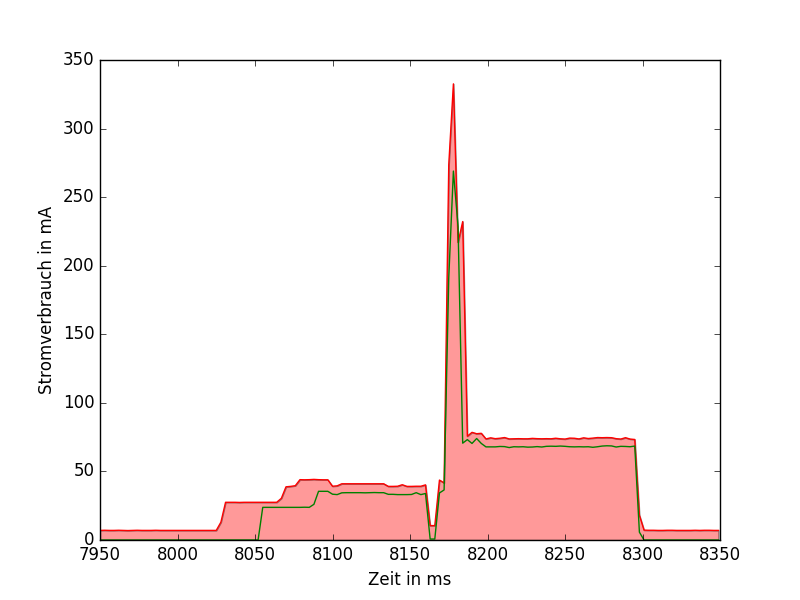
\includegraphics[width=\textwidth]{plots/probereqv.png}
  \caption{Stromverbrauchskurve eines Ortungsvorgangs mit \emph{Probe Requests}.}
  \label{fig:probereqv}
\end{figure}

Beim \emph{ESP8266} Feather misst er jedoch durchgehend einen Vebrauch von über 7 mA, daraus ergeben sich die Unterschiede in den Messungen, die in Tabelle \ref{table:probereqina} dargestellt werden.
Es wurde sowohl mit nur einem versendeten \emph{Probe Request}, als auch mit drei \emph{Probe Requests} getestet, die Unterschiede im Verbrauch liegen jedoch im Bereich der Messungenauigkeit.
Für den normalisierten Stromverbrauch wurde der Verbrauch im Ruhezustand subtrahiert. 
Dies beschränkt den Verbrauch auf den für die tatsächliche Funktion nötigen Anteil.

\begin{table}[h!]
	\centering
	\caption{Stromverbrauch mobiler Einheiten mit \emph{Probe-Request-Lokalisierung}}
	\label{table:probereqina}
	\begin{tabular}{l|p{5.3cm}|R{2.5cm}|R{2.2cm}}
		Hardware & Programm & $\varnothing$ Verbrauch in mA (normalisiert) & Laufzeit in Stunden\\
		\hline
		\emph{ESP8266} Feather & \emph{Probe-Request-Lokalisierung} drei Kanäle & 9,7 (2,7) & 144,0\\
		\emph{ESP-12F} & \emph{Probe-Request-Lokalisierung} drei Kanäle & 1,8 (1,8) & 777,8\\
		\emph{ESP8266} Feather & \emph{Probe-Request-Lokalisierung} ein Kanal & 9,7 (2,7) & 143,7\\
		\emph{ESP-12F} & \emph{Probe-Request-Lokalisierung} ein Kanal & 1,8 (1,8) & 769,2\\
	\end{tabular}
\end{table}

\subsection{Beschleunigungssensor}
\label{ch:Beschleunigungssensor}
Um den Stromverbrauch der \emph{Probe-Request}-basierten Lösung weiter zu senken wird in diesem Abschnitt die Einbindung eines Beschleunigungssensors, in Anlehnung an die kommerzielle Lösung von Ekahau\footnote{\url{https://www.airistaflow.com/}}, diskutiert. 

Im Tunnel Rastatt, in dem auch die Versuche stattfanden, arbeiten die Bauarbeiter in zwei Schichten zu je 12 Stunden. 
Nach 10 Tagen Schicht hat ein Arbeiter 5 Tage frei, jeder Arbeiter arbeitet also genau ein Drittel der Gesamtzeit. 

Die mobile Einheit behält jedoch derzeit seinen Senderythmus bei, angesichts des hohen Stromverbrauchs beim Senden ist dies ineffizient.
Ein Beschleunigungssensor soll bestimmen, wann die mobile Einheit in Bewegung ist. 
Dadurch wird sie nicht mehr senden, wenn sie nicht getragen wird.

\subsubsection{LIS3DH}
Der \emph{LIS3DH} ist ein Drei-Achsen-Beschleunigungssensor von ST Microelectronics \cite{st2015lis}.
Er zeichnet sich durch einen \emph{ultra-low-power} Modus und einen Pin für externe Unterbrechungen (\emph{Interrupt}) aus.
Der Beschleunigungssensor bietet ein \emph{I²C} und ein \emph{SPI Interface}, um ihn zu konfigurieren.
Der \emph{LIS3DH} benötigt bei einer Frequenz von 1 Hz nur 2 \textmu A (0,002 mA).

Leider konnte bei 1 Hz der \emph{Interrupt} durch Laufbewegungen nicht sicher ausgelöst werden, die Frequenz wurde deshalb auf 10 Hz erhöht.
Für eine Frequenz von 10 Hz im \emph{ultra-low-power} Modus listet das Datenblatt einen Verbrauch von 3 \textmu A.
Abbildung \ref{fig:lis3dh} zeigt eine Platine mit integriertem \emph{LIS3DH}.

\begin{figure}[h]
  \centering
	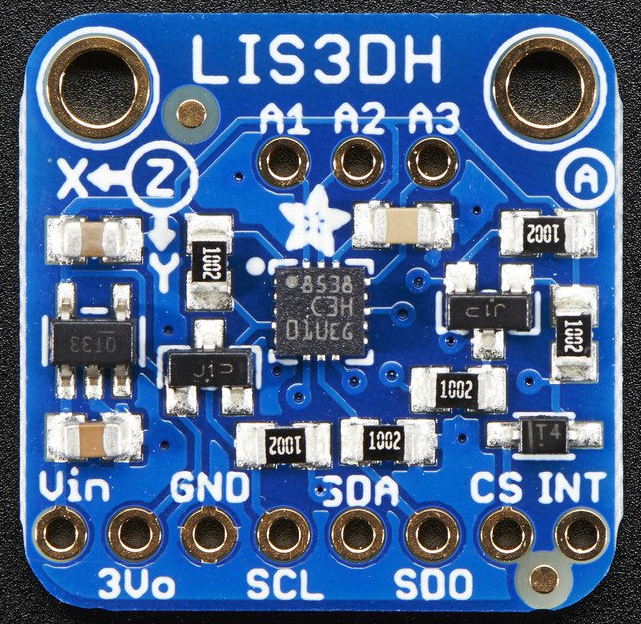
\includegraphics[width=0.5\textwidth]{images/lis3dhada.png}
  \caption{\emph{LIS3DH} integriert auf einer Platine für die Entwicklung. Bild von Adafruit Industries\protect \footnotemark.}
  \label{fig:lis3dh}
\end{figure}
\footnotetext{\url{https://www.adafruit.com/product/2809}}

\subsubsection{Abschaltautomatik}
\label{ch:Beschleunigungssensor:sec:Abschaltautomatik}
Der \emph{ESP8266} besitzt einen \emph{Enable Pin} (CH\_PD), ist dieser mit der Versorungsspannung verbunden, werden die internen Spannungsregler aktiviert und der \emph{ESP8266} mit Strom versorgt.
Die eigentliche Stromversorgung bezieht er dabei jedoch aus dem \emph{Vcc Pin}.
Der \emph{ESP8266} soll durch den \emph{LIS3DH} angeschaltet werden. 
Der \emph{ESP8266} darf die Stromversorgung bei Bedarf trennen, sie kann danach wieder vom \emph{LIS3DH} aktiviert werden. 

Um dieses Verhalten zu erreichen wird ein \emph{Latch} eingesetzt \cite{texas2003latch}.
Es handelt sich dabei um einen digitalen Schalter mit einem SET-Eingang (An), einem RESET-Eingang (Aus) und einem Ausgang.
Der Ausgang wird mit dem \emph{Enable Pin} verbunden, ist er aktiv, wird der \emph{ESP8266} aktiv.
Der SET-Eingang wird mit dem \emph{Interrupt Pin} des \emph{LIS3DH} verbunden, er kann damit den Ausgang aktivieren.
Der RESET-Eingang wird mit dem \emph{ESP8266} verbunden. 
Es wurde \emph{Pin 16} ausgewählt, da dieser für das Aufwecken aus dem Tiefschlaf zuständig ist. 
Stattdessen soll er nun die Stromversorgung abschalten und durch die zuvor im \texttt{deep\_sleep} verbrachte Zeit das Sendeintervall abwarten.

Da das Aufwecken mit \emph{Pin 16} durch das Verbinden des Pins mit der Masse funktioniert, kann damit nicht direkt der RESET-Eingang des Latches betrieben werden.
Stattdessen wird das Ergebnis von \emph{Pin 16} mit der Versorgungsspannung über ein XOR-Gatter verschaltet und mit dem RESET-Eingang verbunden \cite{texas2014xor}.
Abbildung \ref{fig:schematics} zeigt das Schema der Verbindung von \emph{ESP8266} und \emph{LISD3H}.

\begin{figure}[h]
  \centering
	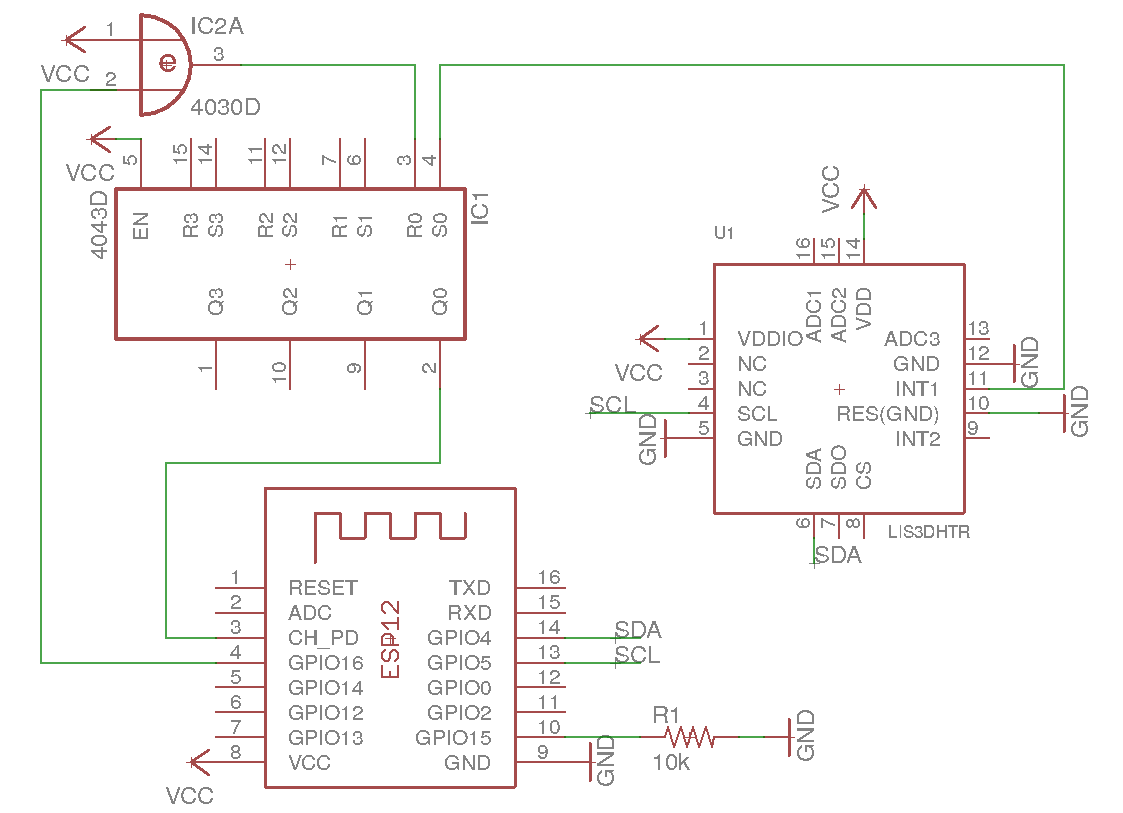
\includegraphics[width=\textwidth]{images/schematics.png}
  \caption{Schema der Verbindung von \emph{ESP8266} und \emph{LIS3DH}.}
  \label{fig:schematics}
\end{figure}

\subsubsection{Bewertung}
Der Verbrauch des Beschleunigungssensors ersetzt lediglich den Verbrauch des Mikrocontrollers, die anderen Komponenten bleiben davon unberührt.
Zu den 3 \textmu A Verbrauch addiert sich deshalb der Verbrauch des Spannungswandlers (55 \textmu A) und des Lithium-Polymer-Ladeschaltkreises (bis zu 100 \textmu A).
Hinzu kommen bis zu 1 \textmu A für das \emph{Latch} und 10 \textmu A für das XOR-Gatter.

Die Integration des Beschleunigungssensor kann also den Verbrauch des \emph{ESP8266} außerhalb der Arbeitszeiten durch einen Verbrauch von 14 \textmu A ersetzen, die bis zu 166 \textmu A Verbrauch der umliegenden Komponenten bleibt jedoch vorhanden.
Die Laufzeit für eine nicht bewegte mobilen Einheit mit \emph{ESP8266} beträgt dann mindestens $1400\ mAh / 0,18\ mA = 7777,77\ h$, dies entspricht ca. 324 Tagen.

Bei den vorherigen Prototypen, die eine \emph{Assoziation} erforderten, muss beachtet werden, dass sie nach dem erneuten Anschalten einen \emph{Scan}- und \emph{Join}-Vorgang ausführen.
Damit diese die Einsparung nicht überwiegen, sollte eine Abschaltung erst nach einigen Minuten der Inaktivität erfolgen.



\section{Direkte Fernlokalisierung mit Bluetooth Low Energy}
\label{ch:phase3}
Für die direkte Fernlokalisierung mit Bluetooth werden dedizierte Basisstationen eingesetzt. 
Die Kommunikation zwischen Basisstation und Ortungsdienst kann durch ein LAN- oder WLAN-Netzwerk gewährleistet werden.
Die Basisstationen bestimmen des \emph{Received Signal Strength Indicator} (RSSI) eingehender Übertragungen der mobilen Enheiten und übermitteln die gemessenen Werte dann an den Ortungsdienst.
Der Ortungsdienst kann mit den gesammelten Werten die Position der mobilen Einheit berechnen.

\subsection{nRF52832}
Der nRF52832 ist eine \emph{System-on-Chip}-Lösung von Nordic Semiconductor.
Er vereint eine 32-bit ARM Cortex-M4F CPU, 512kB RAM und einen 2,4 GHz Transceiver, der Bluetooth 5.0 inklusive Low Energy und das proprietäre ANT Protokoll unterstützt \cite{nordic2017nrf}.

Für diese Arbeit wird ein Adafruit Feather \emph{nRF52} verwendet, der nRF52832 wird deshalb im Folgenden auf \emph{nRF52} abgekürzt.
Das Adafruit Feather \emph{nRF52} besitzt neben dem nRF52832 Spannungswandler für die 3,3 Volt Umwandlung und einen Schaltkreis für die Verwendung mit Lithium Akkus. 
Die verbaute CP2104 USB-to-Serial Schnittstelle erlaubt es, den Chip über USB zu programmieren.

Abbildung \ref{fig:nrf52layout} zeigt das Adafruit Feather nRF52.
Auch Nordic Semiconductor gibt einige typische Stromverbräuche für ihr \emph{System-on-Chip} an, diese sind in Tabelle \ref{table:nrf52consumption} aufgeführt.

\begin{figure}[h]
  \centering
	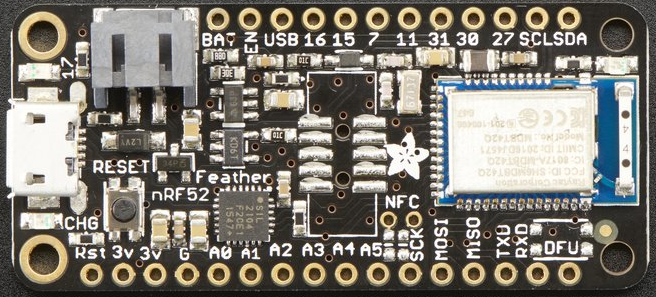
\includegraphics[width=\textwidth]{images/nrf52ada.png}
  \caption{Adafruit \emph{nRF52} Feather. Bild von Adafruit Industries\protect \footnotemark.}
  \label{fig:nrf52layout}
\end{figure}
\footnotetext{\url{https://www.adafruit.com/product/3406}}

\begin{table}[h]
  \centering
  \caption{Stromverbrauch des nRF52832 in verschiedenen Zuständen, aus \cite{nordic2017nrf}}
	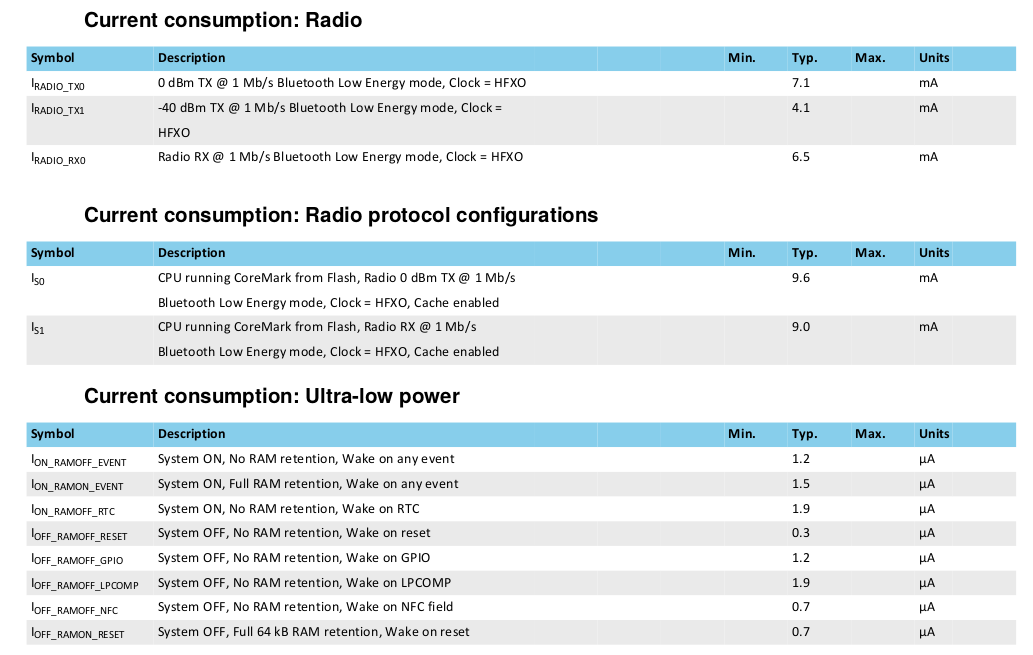
\includegraphics[width=\textwidth]{images/nrf52consumption.png}
  \label{table:nrf52consumption}
\end{table}


\subsubsection{Arduino Bluefruit nRF52 API}
Der \emph{nRF52} kann ebenfalls mit der Arduino IDE programmiert werden.\\
Adafruit stellt eine englischsprachige Anleitung zur Verwendung des \textit{Adafruit Feather nRF52 Bluefruit} mit Arduino zur Verfügung\footnote{\url{https://learn.adafruit.com/bluefruit-nrf52-feather-learning-guide?view=all}}.
Die \emph{Bluefruit nRF52} API stellt dabei Funktionen zur Verwendung von Bluetooth und Bluetooth Low Energy zur Verfügung.
Es wird die \emph{Bluefruit nRF52} API Version 0.6.0 verwendet.



\subsection{Reichweite von Bluetooth Low Energy}
Der Versuch mit BLE wurde an der selben Stelle wie der mit WLAN durchgeführt, siehe dazu Abschitt \ref{ch:phase1:sec:rangewlan}.
Es wurde allerdings ein \emph{Raspberry Pi Zero W} als Basisstation verwendet, dieser wurde auf dem \emph{LN-862} platziert, auf Abbildung \ref{fig:applacement} ist sein rotes Gehäuse zu erkennen.

\subsubsection{Methodik}
Die Reichweite wurde erneut in zwei Richtungen geprüft. 
Zum einen in Richtung der fertig gebohrten Tunnels mit wenigen Hindernissen, zum anderen in Richtung des Vortriebs durch mehrere Stahlhindernisse.
Die zwei Messtrecken werden in Abbildung \ref{fig:rangeblue} skizziert.

\begin{figure}[h!]
  \centering
	\includegraphics[width=\textwidth]{images/rangeblue.eps}
  \caption{Messtrecken zur Festellung der Reichweite von Bluetooth Low Energy.}
  \label{fig:rangeblue}
\end{figure}

Um die Abschirmung durch ein Gehäuse zu simulieren wurde eine stabile Plastikbox verwendet, leider konnte diese nicht vollends geschlossen werden.
Für die Messung wurde der Körper zwischen mobile Einheit und Basisstation gebracht und eine mobile Einheit wurde dann als "`außer Reichweite"' angesehen, wenn versendete Pakete der mobilen Einheit nicht mehr bei der Basisstation ankamen.
Durch das Entfernen des körperlichen Hindernisses war es möglich wieder eine Verbindung herzustellen.

Die bestimmten Reichweiten werden in zwei Meter Schritten angegeben, da sie mit Hilfe der zwei Meter breiten \emph{Tübbinge} bestimmt wurden.

\subsubsection{Ergebnisse}
Tabelle \ref{table:rangeblue} zeigt die Ergebnisse für den nRF52.
Das lose Auflegen des Gehäusedeckels führte zu keiner Veränderung bei der Reichweite.

\begin{table}[h]
	\centering
	\caption{Sendereichweite Bluetooth-basierter mobiler Einheiten}
	\label{table:rangeblue}
	\begin{tabular}{l|l|l|R{3cm}}
		Hardware & Aufbau & Strecke & Maximale Sendereichweite \\
		\hline
		\emph{nRF52} Feather & Offen & Wenige Hindernisse & 32 m \\
		\emph{nRF52} Feather & In Gehäuse & Wenige Hindernisse & 32 m \\
		\emph{nRF52} Feather & Offen & Viele Hindernisse & 14 m \\
		\emph{nRF52} Feather & In Gehäuse & Viele Hindernisse & 14 m \\
	\end{tabular}
\end{table}

\subsubsection{Bewertung}
Um mit 30 km/h 32 Meter zu durchqueren benötigt man 3,8 Sekunden.
Da jedoch eine hohe Erkennungszuverlässigkeit gefordert wurde, sollte das Sendeintervall niedriger gesetzt werden, es wird auf eine Sekunde gesetzt.
Damit werden auch bei einer Reichweite von nur 14 Metern auf der Tunnelbohrmaschine ausreichend viele Pakete versenden um den Verlust einzelner zu kompensieren.

\subsection{BLE-Advertising-Implementierung}
\label{ch:phase3:sec:advertising}
Die \emph{Bluetooth-Low-Energy-Implementierung} ist an die Arbeit von Jianyong et al. angelehnt.
Es wird immer nach Ablauf des Sendeintervalls ein \emph{Advertising} Paket gesendet.

In der Praxis wird dazu das \emph{Advertising}-Intervall entsprechend gesetzt, dabei handelt es sich um einen in Bluetooth 4.0 spezifizierten Parameter für die Häufigkeit des \emph{Advertisings}.
Da die \emph{Bluefruit} \emph{nRF52} API keine Funktion zur Änderung dieses Wertes zur Verfügung stellt muss er direkt geändert werden.
Die entsprechende \emph{BLEAdvertising}-Klasse ist in \\\texttt{/.arduino15/packages/adafruit/hardware/nrf52/0.6.0/libraries/}\\\texttt{Bluefruit52Lib/src} zu finden. 

In \texttt{BLEAdvertising.cpp} ist \texttt{GAP\_ADV\_INTERVAL\_MS} auf 20 Millisekunden gesetzt, dieser Wert sollte erhöht werden, um den Stromverbrauch zu senken.
Beim \emph{nRF52} handelt es sich um ein Klasse 2 Bluetooth-Gerät mit einer maximalen Sendeleistung bis 4 dBm.
Das Sendeintervall wird etsprechend der Untersuchung der Reichweite und maximalen Bewegungsgeschwindigkeit von 30 km/h auf eine Sekunde gesetzt, in dieser Zeit kann sich ein Mitarbeiter maximal 9 Meter bewegen.

Es sollte erneut eine Voruntersuchung des Verbrauchs mit dem Muker \emph{TM103} USB-Power-Meter vorgenommen werden.
Diser ist aber nicht in der Lage den Stromverbrauch des \emph{nRF52} zu messen.
Die Sendeabschnitte sind zu kurz um einen messbaren Stromverbrauch zu erzeugen.

Deshalb wird zunächst Abbildung \ref{table:nrf52consumption} für eine theoretische Betrachtung des Verbrauchs herangezogen werden. 




\subsection{Untersuchung des Stromverbrauchs}
Der Stromverbrauch soll mit dem INA219 genauer bestimmt werden, der INA219 und die verwendete Methodik werden in Abschnitt \ref{ch:phase1:sec:energie} beschrieben.

\subsubsection{Theoretische Stromverbrauchsabschätzung}
Für die Zeit in der nicht gesendet wird, wird der Zustand $I_{ON\_RAMOFF\_RTC}$ angenommen, da dieser den höchsten Verbrauch aufweist.
Für die Sendezeit wird $I_{RADIO\_TX0}$ angenommen, für ein \emph{Advertising}-Paket, welches zusätzlich den Gerätenamen "`TestTag"' versendet, werden 24 Bytes (192 Bit) gesendet.
Um die Kollisionsvermeidung einzufügen werden vorher 2000 Bit im Zustand $I_{RADIO\_RX0}$ empfangen, der die restliche Zeit wird in $I_{ON\_RAMOFF\_RTC}$ verbracht. 
Es müssen ebenfalls die weiteren Komponenten auf dem Feather bedacht werden. 
Adafruit gibt für den Spannungswandler einen Verbrauch von 55 \textmu A und für den Lithium-Polymer-Ladeschaltkreis einen Verbrauch von bis zu 100 \textmu A an \cite{fried2016lora}. 
Der Verbrauch des anderen Komponenten des Feather wird daher konservativ auf 155 \textmu A geschätzt.
Damit ergibt sich ein durchschnittlicher Verbrauch $y$ in Höhe von: 

$y = (1s-\frac{Bits\_gesendet}{1000000 b/s} - \frac{Bits\_empfangen}{1000000 b/s}) * (I_{ON\_RAMOFF\_RTC} + 155 {\mu}A) + \frac{Bits\_gesendet}{1000000 b/s} * I_{RADIO\_RX0} + \frac{Bits\_empfangen}{1000000 b/s} * I_{RADIO\_RX0}$

$y = (1s - 0,000192s - 0,002s) * 0,1569mA + 0,000192 * 7,1mA + 0,002 * 6,5mA$

$y \approx 0,156556mA + 0,001363mA + 0,013mA = 0,170919mA$ 

\subsubsection{Tatsächlicher Stromverbrauch von BLE}
\label{ch:phase3:sec:powerble}
Abbildung \ref{fig:blue} zeigt den Lastverlauf für den Start einer mobilen Einheit mit Bluetooth-Low-Energy-Advertising.

Zu Beginn ist eine Startphase zu erkennen, ab 2 Sekunden nach Start des Experiments ist dann das regelmäßige Muster aus Verbrauch im Ruhezustand und kurzen Verbrauchsspitzen beim Senden zu erkennen.
Die Kürze des Sendevorgangs bedingt die starke Schwankung bei den Lastspitzen, die Samplingrate von 333 Hz reicht hier offenbar nicht aus um dem Sendevorgang vollständig zu erfassen.

\begin{figure}[h!]
  \centering
	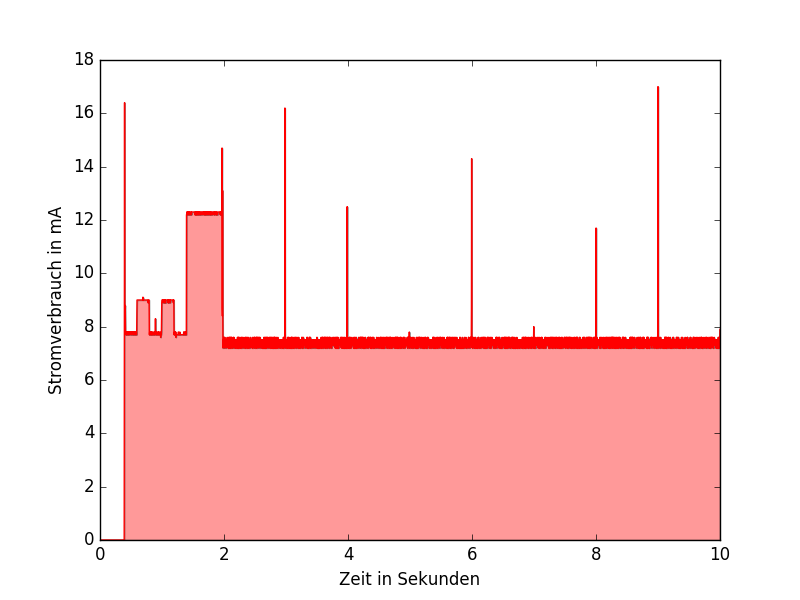
\includegraphics[width=\textwidth]{plots/blue.png}
  \caption{Stromverbrauchskurve einer Implementierung von Bluetooth-Low-Energy-Advertising.}
  \label{fig:blue}
\end{figure}

Hauptverbrauch liegt jedoch in den 7,2 bis 7,6 mA im Ruhezustand, leider ist in diesem Fall kein einzelnes Modul vorhanden, es kann nur auf dem \emph{nRF52} Feather gemessen werden.
Tabelle \ref{table:blueina} zeigt deshalb neben dem gemessenen Verbrauch den normalisierten Stromverbrauch, dafür wurde der Verbrauch im Ruhezustand subtrahiert. 
Dies beschränkt den Verbrauch auf den für die tatsächliche Funktion nötigen Anteil.

\begin{table}[h!]
	\centering
	\caption{Stromverbrauch mobiler Einheiten mit Bluetooth-Low-Energy-Advertising}
	\label{table:blueina}
	\begin{tabular}{p{3.5cm}|p{5cm}|R{2.5cm}|R{2.5cm}}
		Hardware & Programm & $\varnothing$ Verbrauch in mA (normalisiert) & Laufzeit in Stunden\\
		\hline
		\emph{nRF52} Feather & Bluetooth-Low-Energy-Advertising & 7,37 (0,04) & 190\\
	\end{tabular}
\end{table}




%% ++++++++++++++++++++++++++++++++++++++++++
%% Anhang
%% ++++++++++++++++++++++++++++++++++++++++++

\appendix
%\include{anhang_a}
%\include{anhang_b}

%% ++++++++++++++++++++++++++++++++++++++++++
%% Literatur
%% ++++++++++++++++++++++++++++++++++++++++++
%  mit dem Befehl \nocite werden auch nicht 
%  zitierte Referenzen abgedruckt
\cleardoublepage
\phantomsection
\addcontentsline{toc}{chapter}{\bibname}
%%
\nocite{*} % nur angeben, wenn auch nicht im Text zitierte Quellen 
           % erscheinen sollen
\bibliographystyle{itmabbrv} % mit abgekürzten Vornamen der Autoren
%\bibliographystyle{gerplain} % abbrvnat unsrtnat
% spezielle Zitierstile: Labels mit vier Buchstaben und Jahreszahl
%\bibliographystyle{itmalpha}  % ausgeschriebene Vornamen der Autoren
\bibliography{thesis}
%% ++++++++++++++++++++++++++++++++++++++++++
%% Index
%% ++++++++++++++++++++++++++++++++++++++++++
\ifnotdraft{
\cleardoublepage
\phantomsection
\printindex            % Index, Stichwortverzeichnis
}
\end{document}
%% end of file
